\documentclass[preprint,aps,pra,onecolumn]{revtex4-1} %reprint
%\tightenlines

%\draft
\usepackage{etex}
\usepackage{amsmath}
\usepackage{bm}
\usepackage{bbm}
\usepackage{listings}
% % \textwidth 16cm \textheight 23.5cm
% \renewcommand{\baselinestretch}{1.2}
\usepackage{graphicx}
\usepackage{graphics}
\usepackage{epsfig}
\usepackage{color}
\usepackage{multirow}
\usepackage[colorlinks]{hyperref}
\usepackage{fancyhdr}
\usepackage{calc}
\usepackage{natbib} %[numbers]
\usepackage{bibentry}
% underline tool
\usepackage[normalem]{ulem}
\usepackage{xcolor}
%\uline{foo}	Underlines foo
%\uuline{foo}	Double underlines foo
%\uwave{foo}	Underlines foo with a wavy line
%\sout{foo}	Strikesout foo
%\xout{foo}	Crosses out foo with ¡®/6¤7¡¯
% triple lines in colors
\makeatletter
\newcommand\uuuline{\bgroup\markoverwith%
   {%
     \textcolor{red}{\rule[-0.5ex]{2pt}{0.4pt}}%
     \llap{\textcolor{blue}{\rule[-0.7ex]{2pt}{0.4pt}}}%
     \llap{\textcolor{green}{\rule[-0.9ex]{2pt}{0.4pt}}}%
   }%
   \ULon}
\makeatother


\usepackage{amsmath,soul} % underline with a number
% usage example: $\underset{4}{\text{\ul{This is short text}}}$
% another package to use, but did not work for me.
% From: http://tex.stackexchange.com/questions/45341/labeling-underlined-text-over-multiple-lines
%\usepackage{soulpos}
%\ulposdef{\ulnumaux}{%
%   $\underset{\saveulnum}{\rule[-.7ex]{\ulwidth}{.4pt}}$}
%
%\newcommand{\ulnum}[2]{%
%  \def\saveulnum{#1}%
%  \ulnumaux{#2}}

% todo list and commands
\usepackage{todonotes}
%% to avoid the conflict with amths package % not working
%\makeatletter
%\providecommand\@dotsep{5}
%\makeatother
%\listoftodos\relax
\usepackage{makeidx}
\allowdisplaybreaks
% for eps transfering to pdf.
\usepackage[update,prepend]{epstopdf}
\usepackage{ifpdf}

\ifpdf
   \usepackage{graphicx}
   \usepackage{epstopdf}
   \epstopdfsetup{suffix=}
   \DeclareGraphicsRule{.eps}{pdf}{.pdf}{`epstopdf #1}
   \pdfcompresslevel=9
\else
   \usepackage{graphicx}
\fi
% subfig
\usepackage{mwe}
\usepackage{subfig}
% to fix a figure's position using [H] option of thec figure.
\usepackage{float}
% to use \lesssim and other math symbols
\usepackage{amssymb}


% self-defined short-cuts and commands

% packages we need for judging the operating system
% compile your tex file with option -shell-escape is required: 
% e.g. xelatex -shell-escape file.tex
\usepackage{pdftexcmds}
\usepackage{catchfile}
\usepackage{ifluatex}
\usepackage{ifplatform}

% self-definition for short hand

% symbols and math operators
\DeclareMathOperator{\spn}{span}
\DeclareMathOperator{\tr}{tr}
% definition of grammars % formats related
\definecolor{MyDarkGreen}{rgb}{0.0,0.4,0.0}
\newcommand{\greek}[1]{{\selectlanguage{greek}#1}} % will look for grmn font: tlmgr install cbfonts (65 MB)

% functions
\newcommand{\sn}{\mathrm{sn}}
\newcommand{\cn}{\mathrm{cn}}
\newcommand{\dn}{\mathrm{dn}}

% constants
\newcommand{\invtpi}{\frac{1}{2\pi}}

% vectors and tensors
\def\en{\mathbf{e}_n}
\def\eye{\mathbf{I}}
\newcommand\lvec[1]{\accentset{\leftarrow}{#1}}
% math font
\newcommand{\bmc}[1]{\boldsymbol{\mathcal{#1}}}

% derivatives and integrals
% ordinary derivatives
\newcommand{\drv}{\mathrm{d}}
\newcommand{\dt}[1]{\frac{{\mathrm d} {#1}}{{\mathrm d}t}}
\newcommand{\dx}[1]{\frac{{\mathrm d} {#1}}{{\mathrm d}x}}
\newcommand{\dtau}{\frac{{\mathrm d} }{{\mathrm d}\tau}}
\newcommand{\dd}[2]{\frac{{\mathrm d} {#1}}{{\mathrm d} {#2}}}
\newcommand{\sdt}[1]{\frac{{\mathrm d}^2 {#1}}{{\mathrm d}t^2}}
\newcommand{\sdx}[1]{\frac{{\mathrm d}^2 {#1}}{{\mathrm d}x^2}}
\newcommand{\sdd}[2]{\frac{{\mathrm d}^2 {#1}}{{\mathrm d}{#2}^2}}
\newcommand{\ddn}[3]{\frac{{\mathrm d}^{#1} #2}{{\mathrm d} #3 ^{#1}}}

% partial derivatives
\newcommand{\pt}[1]{\frac{\partial {#1}}{\partial t}}
\newcommand{\px}[1]{\frac{\partial {#1}}{\partial x}}
\newcommand{\pp}[2]{\frac{\partial {#1}}{\partial {#2}}}
\newcommand{\spt}[1]{\frac{\partial^2 {#1}}{\partial t^2}}
\newcommand{\spx}[1]{\frac{\partial^2 {#1}}{\partial x^2}}
\newcommand{\spp}[2]{\frac{\partial^2 {#1}}{\partial {#2}^2}}
\newcommand{\ppn}[3]{\frac{\partial^{#1} #2}{\partial #3 ^{#1}}}
% integrals
\newcommand{\intl}[2]{\int_0^\infty\! #1 \mathrm{d}#2}
\newcommand{\intf}[2]{\int_{-\infty}^\infty\! #1 \mathrm{d}#2}


% quantum operators
\newcommand{\ssp}{\braket{\sigma^{+}(t)\sigma^{-}(t)}}
\newcommand{\aap}{\braket{a^{\dagger}(t)a(t)}}
\newcommand{\as}{\braket{a^{\dagger}(t)\sigma^{-}(t)}}
\newcommand{\sa}{\braket{a(t)\sigma^{+}(t)}}
\newcommand{\Hssp}{\braket{\sigma^{+}\sigma^{-}}}
\newcommand{\Haap}{\braket{a^{\dagger}a}}
\newcommand{\Has}{\braket{a^{\dagger}\sigma^{-}}}
\newcommand{\Hsa}{\braket{a\sigma^{+}}}
\newcommand{\adag}{a^{\dagger}}
\newcommand{\sigm}{\sigma^{-}}
\newcommand{\sigp}{\sigma^{+}}
\newcommand{\sigz}{\sigma^{z}}
\newcommand{\gp}{\gamma^{\prime}}
\newcommand{\oal}{\omega_a-\omega_0}
\newcommand{\ocl}{\omega_c-\omega_0}


% Green function related
\def\GFT{\overline{\bf G}}
\def\IT{\overline{\bf I}}
\def\TT{\overline{\bf T}}
\def\MT{\overline{\bf M}}
\def\AT{\overline{\bf A}}
\def\BT{\overline{\bf B}}
\def\fT{\overline{\bf f}}
\def\LT{\overline{\bf L}}
\def\alphaT{\overline{\bf \alpha}}
\def\GFTr{\overline{\bf G}\left(\mathbf{r},\mathbf{r}'\right)}
\def\GFTrw{\overline{\bf G}\left(\mathbf{r},\mathbf{r}';\omega\right)}
\def\rarg{\left(\mathbf{r}\right)}
\def\rargw{\left(\mathbf{r};\omega\right)}
\def\rrarg{\left(\mathbf{r},\mathbf{r}'\right)}
\def\rrargw{\left(\mathbf{r},\mathbf{r}';\omega\right)}
\def\rk{\left(\mathbf{r}_k\right)}
\def\rn{\left(\mathbf{r}_n\right)}
\def\rnrn{\left(\mathbf{r}_n,\mathbf{r}_n\right)}
\def\rnrk{\left(\mathbf{r}_n,\mathbf{r}_k\right)}
\def\rkrk{\left(\mathbf{r}_k,\mathbf{r}_k\right)}
\def\rkrn{\left(\mathbf{r}_k,\mathbf{r}_n\right)}
\def\br{\mathbf{r}}
\def\Erw{\hat{\mathbf{E}}(\mathbf{r},\omega)}
\def\E0{\hat{\mathbf{E}}^{(0)}(\mathbf{r},\omega)}
\def\Arw{\hat{\mathbf{A}}(\mathbf{r},\omega)}
\def\Snw{\hat{\mathbf{S}}_n(\omega)}
\def\Unw{\mathbf{U}_n(\omega)}
\def\unw{U_n(\omega)}
\def\Alphanw{{\bm \alpha}_n(\omega)}
\def\Krrw{\mathbf{K}(\mathbf{r},\mathbf{r}',\omega)}
\def\Krrnw{\mathbf{K}(\mathbf{r},\mathbf{r}_n,\omega)}
\def\GTrrw{\mathbf{G}^T(\mathbf{r},\mathbf{r}',\omega)}
\def\Grrw{\mathbf{G}(\mathbf{r},\mathbf{r}',\omega)}
\def\Gn{\mathbf{G}^n}
\def\Gm1{\mathbf{G}^{n-1}}
\def\GN{\mathbf{G}^N}
\def\G0{\mathbf{G}^0}
\def\G1{\mathbf{G}^1}
\def\Gi{\mathbf{G}^i}
\def\flamr{\mathbf{f}_\lambda(\mathbf{r})}
\def\rrn{\mathbf{r},\mathbf{r}_n}
\def\rnrn{\mathbf{r}_n,\mathbf{r}_n}
\def\rr{\mathbf{r},\mathbf{r}'}


% braket.sty          Macros for Dirac bra-ket <|> notation and sets {|}
%
\def\bra#1{\langle{#1}\rvert}%{\mathinner{\langle{#1}\rvert}}
\def\ket#1{\lvert{#1}\rangle}%{\mathinner{\lvert{#1}\rangle}}
\def\braket#1{\mathinner{\langle{#1}\rangle}}
\def\Bra#1{\left<#1\right|}
\def\Ket#1{\left|#1\right>}
{\catcode`\|=\active
  \gdef\Braket#1{\left<\mathcode`\|"8000\let|\BraVert {#1}\right>}}
\def\BraVert{\egroup\,\mid@vertical\,\bgroup}
{\catcode`\|=\active
  \gdef\set#1{\mathinner{\lbrace\,{\mathcode`\|"8000\let|\midvert #1}\,\rbrace}}
  \gdef\Set#1{\left\{\:{\mathcode`\|"8000\let|\SetVert #1}\:\right\}}}
\def\midvert{\egroup\mid\bgroup}
\def\SetVert{\egroup\;\mid@vertical\;\bgroup}
% Some stuff deleted
% Macros for Dirac bra-ket <|> notation
%\def\bra#1{\mathinner{\langle{#1}|}}
%\def\ket#1{\mathinner{|{#1}\rangle}}
\def\Braket#1#2{\mathinner{\langle{#1}\! \mid\! {#2} \rangle}}
\def\ketbra#1{\ket{#1}\!\!\bra{#1}}
\newcommand{\Ketbra}[2]{\ket{#1}\!\!\bra{#2}}
\def\sandwich#1#2{\bra{#1}\! #2 \! \ket{#1}}
\def\Sandwich#1#2#3{\bra{#1}\! #2\! \ket{#3}}
%
% END  braket.sty     Macros for Dirac bra-ket <|> notation and sets {|}


%% Ben's shortcuts.
% Equation, citation, and labeling macros
%========================================================================================
\newcommand{\erf}[1]{Eq.~(\ref{#1})}
\newcommand{\frf}[1]{Fig.~\ref{#1}}
\newcommand{\srf}[1]{Sec.~\ref{#1}}
\newcommand{\nn}{\nonumber}
\newcommand{\mbf}[1]{\mathbf{#1}}
%========================================================================================
% General quantum mechanics macros
%========================================================================================
\newcommand{\ip}[2]{\langle{#1}|{#2}\rangle}
\newcommand{\op}[2]{\ket{#1}\bra{#2}}
\newcommand{\enavg}[1]{\mathrm{E}\sq{#1}}
\newcommand{\gravg}[1]{\mathbb{E}\sq{#1}}
\newcommand{\expt}[1]{\langle{#1}\rangle}
\newcommand{\dg}{^\dagger}
\newcommand{\smallfrac}[2]{\mbox{$\frac{#1}{#2}$}}
\newcommand{\emn}[1]{ \mathbbm{E}_{#1} }
\newcommand{\Tr}{\mbox{Tr}}
%\newcommand{\tensor}[1]{\boldsymbol{#1}}%{\overset{\leftrightarrow}{#1}}
%========================================================================================
% Famous physicists
%========================================================================================
\newcommand{\sch}{Schr\"odinger}
\newcommand{\hei}{Heisenberg }
\newcommand{\ein}{Einstein }
\newcommand{\str}{Stratonovich }
%========================================================================================
% Dirac notation and commutators
%========================================================================================
\newcommand{\norm}[1]{\lvert #1 \rvert}
\newcommand{\opnorm}[1]{\lVert #1 \rVert}
%\newcommand{\ket}[1]{\lvert #1 \rangle}
%\newcommand{\bra}[1]{\langle #1 \rvert}
\newcommand{\bravket}[2]{\langle\, #1\,\vert\, #2 \,\rangle}
\newcommand{\av}[1]{\left\langle #1 \right\rangle}
\newcommand{\proj}[1]{\ket{#1}\!\bra{#1}}
\newcommand{\commut}[2]{[\ssp #1,\,#2\ssp]}
\newcommand{\anticommut}[2]{\{\ssp #1,\,#2\ssp\}}
% big Dirac notation and commutators
\newcommand{\bnorm}[1]{\big\lvert #1 \big\rvert}
\newcommand{\bopnorm}[1]{\big\lVert #1 \big\rVert}
\newcommand{\bket}[1]{\big\lvert\, #1\, \big\rangle}
\newcommand{\bbra}[1]{\big\langle\, #1\, \big\rvert}
\newcommand{\bbraket}[2]{\big\langle\, #1\,\big\vert\, #2 \,\big\rangle}
\newcommand{\bav}[1]{\bigl\langle #1 \bigr\rangle}
\newcommand{\bproj}[1]{\bket{#1}\!\bbra{#1}}
\newcommand{\bcommut}[2]{\big[\ssp #1,\,#2\ssp\big]}
\newcommand{\banticommut}[2]{\big\{\ssp #1,\,#2\ssp\big\}}
% Big Dirac notation and commutators
\newcommand{\Bnorm}[1]{\Big\lvert #1 \Big\rvert}
\newcommand{\Bopnorm}[1]{\Big\lVert #1 \Big\rVert}
\newcommand{\Bket}[1]{\Big\lvert\, #1\, \Big\rangle}
\newcommand{\Bbra}[1]{\Big\langle\, #1\, \Big\rvert}
\newcommand{\Bbraket}[2]{\Big\langle\, #1\,\Big\vert\, #2 \,\Big\rangle}
\newcommand{\Bav}[1]{\Bigl\langle #1 \Bigr\rangle}
\newcommand{\Bproj}[1]{\Bket{#1}\!\Bbra{#1}}
\newcommand{\Bcommut}[2]{\Big[\ssp #1,\,#2\ssp\Big]}
\newcommand{\Banticommut}[2]{\Big\{\ssp #1,\,#2\ssp\Big\}}
%========================================================================================
% Nanofiber interface macros
%========================================================================================
\newcommand{\expect}[1]{\big\langle #1 \big\rangle}
\newcommand{\expects}[1]{\langle #1 \rangle}
\newcommand{\melement}[3]{\langle #1 \lvert #2 \rvert #3 \rangle}
\newcommand{\Ip}[2]{\left\langle {#1},{#2} \right\rangle}
\newcommand{\modsq}[1]{\lvert #1 \rvert^2}
\newcommand{\normsq}[1]{\lVert #1 \rVert^2}
\newcommand{\grad}{\nabla}
\newcommand{\partialD}[2]{\frac{\partial #1}{\partial #2}}

\newcommand{\peakprobe}{\mathcal{E}_0}
\newcommand{\eff}{\text{eff}}
\newcommand{\varFz}{\big( \Delta F_z^{0} \big)^2}
\newcommand{\varFzText}{( \Delta F_z^{0} )^2}
\newcommand{\varFzLG}{( \Delta F_z^{00} )^2}

\newcommand{\rperp}{\mathbf{r}_\perp}
\newcommand{\talphan}{\overset{\leftrightarrow}{\alpha}{}^{(n)}}
\newcommand{\talphanOp}{\hat{\overset{\leftrightarrow}{\alpha}}{}^{(n)}}

%\newcommand{\Cstrength}{ \chi^{(1)}\sqrt{ \dot{N}_L } }
%\newcommand{\CstrengthSq}{ \big(\chi^{(1)} \big)^2 \dot{N}_L }
\newcommand{\Cstrength}{ \sqrt{\kappa} }
\newcommand{\CstrengthSq}{ \kappa }
%========================================================================================
%  Spacing macros
%========================================================================================
%\newcommand{\ssp}{\hspace{0.4pt}}%small horizontal space
\newcommand{\nsp}{\hspace{-0.7pt}}%negative horizontal space
%========================================================================================




% For faster processing, load Matlab syntax for listings
\lstloadlanguages{Matlab}% use listings package
\lstset{language=Matlab,
        frame=single,
        basicstyle=\small\ttfamily,
        keywordstyle=[1]\color{Blue}\bf,
        keywordstyle=[2]\color{Purple},
        keywordstyle=[3]\color{Blue}\underbar,
        identifierstyle=,
        commentstyle=\usefont{T1}{pcr}{m}{sl}\color{MyDarkGreen}\small,
        stringstyle=\color{Purple},
        showstringspaces=false,
        tabsize=5,
        % Put standard MATLAB functions not included in the default
        % language here
        morekeywords={xlim,ylim,var,alpha,factorial,poissrnd,normpdf,normcdf},
        % Put MATLAB function parameters here
        morekeywords=[2]{on, off, interp},
        % Put user defined functions here
        morekeywords=[3]{FindESS},
        morecomment=[l][\color{Blue}]{...},
        numbers=left,
        firstnumber=1,
        numberstyle=\tiny\color{Blue},
        stepnumber=5
        }
        
        
        
% Includes a figure
% The first parameter is the label, which is also the name of the figure
%   with or without the extension (e.g., .eps, .fig, .png, .gif, etc.)
%   IF NO EXTENSION IS GIVEN, LaTeX will look for the most appropriate one.
%   This means that if a DVI (or PS) is being produced, it will look for
%   an eps. If a PDF is being produced, it will look for nearly anything
%   else (gif, jpg, png, et cetera). Because of this, when I generate figures
%   I typically generate an eps and a png to allow me the most flexibility
%   when rendering my document.
% The second parameter is the width of the figure normalized to column width
%   (e.g. 0.5 for half a column, 0.75 for 75% of the column)
% The third parameter is the caption.
\newcommand{\scalefig}[3]{
  \begin{figure}[ht!]
    % Requires \usepackage{graphicx}
    \centering
    \includegraphics[width=#2\columnwidth]{#1}
    %%% I think \captionwidth (see above) can go away as long as
    %%% \centering is above
    %\captionwidth{#2\columnwidth}%
    \caption{#3}
    \label{#1}
  \end{figure}}
% judge platform and include correct definiation package
%\ifwindows
%	%% self-definition for short hand

% symbols and math operators
\DeclareMathOperator{\spn}{span}
\DeclareMathOperator{\tr}{tr}
% definition of grammars % formats related
\definecolor{MyDarkGreen}{rgb}{0.0,0.4,0.0}
\newcommand{\greek}[1]{{\selectlanguage{greek}#1}} % will look for grmn font: tlmgr install cbfonts (65 MB)

% functions
\newcommand{\sn}{\mathrm{sn}}
\newcommand{\cn}{\mathrm{cn}}
\newcommand{\dn}{\mathrm{dn}}

% constants
\newcommand{\invtpi}{\frac{1}{2\pi}}

% vectors and tensors
\def\en{\mathbf{e}_n}
\def\eye{\mathbf{I}}
\newcommand\lvec[1]{\accentset{\leftarrow}{#1}}
% math font
\newcommand{\bmc}[1]{\boldsymbol{\mathcal{#1}}}

% derivatives and integrals
% ordinary derivatives
\newcommand{\drv}{\mathrm{d}}
\newcommand{\dt}[1]{\frac{{\mathrm d} {#1}}{{\mathrm d}t}}
\newcommand{\dx}[1]{\frac{{\mathrm d} {#1}}{{\mathrm d}x}}
\newcommand{\dtau}{\frac{{\mathrm d} }{{\mathrm d}\tau}}
\newcommand{\dd}[2]{\frac{{\mathrm d} {#1}}{{\mathrm d} {#2}}}
\newcommand{\sdt}[1]{\frac{{\mathrm d}^2 {#1}}{{\mathrm d}t^2}}
\newcommand{\sdx}[1]{\frac{{\mathrm d}^2 {#1}}{{\mathrm d}x^2}}
\newcommand{\sdd}[2]{\frac{{\mathrm d}^2 {#1}}{{\mathrm d}{#2}^2}}
\newcommand{\ddn}[3]{\frac{{\mathrm d}^{#1} #2}{{\mathrm d} #3 ^{#1}}}

% partial derivatives
\newcommand{\pt}[1]{\frac{\partial {#1}}{\partial t}}
\newcommand{\px}[1]{\frac{\partial {#1}}{\partial x}}
\newcommand{\pp}[2]{\frac{\partial {#1}}{\partial {#2}}}
\newcommand{\spt}[1]{\frac{\partial^2 {#1}}{\partial t^2}}
\newcommand{\spx}[1]{\frac{\partial^2 {#1}}{\partial x^2}}
\newcommand{\spp}[2]{\frac{\partial^2 {#1}}{\partial {#2}^2}}
\newcommand{\ppn}[3]{\frac{\partial^{#1} #2}{\partial #3 ^{#1}}}
% integrals
\newcommand{\intl}[2]{\int_0^\infty\! #1 \mathrm{d}#2}
\newcommand{\intf}[2]{\int_{-\infty}^\infty\! #1 \mathrm{d}#2}


% quantum operators
\newcommand{\ssp}{\braket{\sigma^{+}(t)\sigma^{-}(t)}}
\newcommand{\aap}{\braket{a^{\dagger}(t)a(t)}}
\newcommand{\as}{\braket{a^{\dagger}(t)\sigma^{-}(t)}}
\newcommand{\sa}{\braket{a(t)\sigma^{+}(t)}}
\newcommand{\Hssp}{\braket{\sigma^{+}\sigma^{-}}}
\newcommand{\Haap}{\braket{a^{\dagger}a}}
\newcommand{\Has}{\braket{a^{\dagger}\sigma^{-}}}
\newcommand{\Hsa}{\braket{a\sigma^{+}}}
\newcommand{\adag}{a^{\dagger}}
\newcommand{\sigm}{\sigma^{-}}
\newcommand{\sigp}{\sigma^{+}}
\newcommand{\sigz}{\sigma^{z}}
\newcommand{\gp}{\gamma^{\prime}}
\newcommand{\oal}{\omega_a-\omega_0}
\newcommand{\ocl}{\omega_c-\omega_0}


% Green function related
\def\GFT{\overline{\bf G}}
\def\IT{\overline{\bf I}}
\def\TT{\overline{\bf T}}
\def\MT{\overline{\bf M}}
\def\AT{\overline{\bf A}}
\def\BT{\overline{\bf B}}
\def\fT{\overline{\bf f}}
\def\LT{\overline{\bf L}}
\def\alphaT{\overline{\bf \alpha}}
\def\GFTr{\overline{\bf G}\left(\mathbf{r},\mathbf{r}'\right)}
\def\GFTrw{\overline{\bf G}\left(\mathbf{r},\mathbf{r}';\omega\right)}
\def\rarg{\left(\mathbf{r}\right)}
\def\rargw{\left(\mathbf{r};\omega\right)}
\def\rrarg{\left(\mathbf{r},\mathbf{r}'\right)}
\def\rrargw{\left(\mathbf{r},\mathbf{r}';\omega\right)}
\def\rk{\left(\mathbf{r}_k\right)}
\def\rn{\left(\mathbf{r}_n\right)}
\def\rnrn{\left(\mathbf{r}_n,\mathbf{r}_n\right)}
\def\rnrk{\left(\mathbf{r}_n,\mathbf{r}_k\right)}
\def\rkrk{\left(\mathbf{r}_k,\mathbf{r}_k\right)}
\def\rkrn{\left(\mathbf{r}_k,\mathbf{r}_n\right)}
\def\br{\mathbf{r}}
\def\Erw{\hat{\mathbf{E}}(\mathbf{r},\omega)}
\def\E0{\hat{\mathbf{E}}^{(0)}(\mathbf{r},\omega)}
\def\Arw{\hat{\mathbf{A}}(\mathbf{r},\omega)}
\def\Snw{\hat{\mathbf{S}}_n(\omega)}
\def\Unw{\mathbf{U}_n(\omega)}
\def\unw{U_n(\omega)}
\def\Alphanw{{\bm \alpha}_n(\omega)}
\def\Krrw{\mathbf{K}(\mathbf{r},\mathbf{r}',\omega)}
\def\Krrnw{\mathbf{K}(\mathbf{r},\mathbf{r}_n,\omega)}
\def\GTrrw{\mathbf{G}^T(\mathbf{r},\mathbf{r}',\omega)}
\def\Grrw{\mathbf{G}(\mathbf{r},\mathbf{r}',\omega)}
\def\Gn{\mathbf{G}^n}
\def\Gm1{\mathbf{G}^{n-1}}
\def\GN{\mathbf{G}^N}
\def\G0{\mathbf{G}^0}
\def\G1{\mathbf{G}^1}
\def\Gi{\mathbf{G}^i}
\def\flamr{\mathbf{f}_\lambda(\mathbf{r})}
\def\rrn{\mathbf{r},\mathbf{r}_n}
\def\rnrn{\mathbf{r}_n,\mathbf{r}_n}
\def\rr{\mathbf{r},\mathbf{r}'}


% braket.sty          Macros for Dirac bra-ket <|> notation and sets {|}
%
\def\bra#1{\langle{#1}\rvert}%{\mathinner{\langle{#1}\rvert}}
\def\ket#1{\lvert{#1}\rangle}%{\mathinner{\lvert{#1}\rangle}}
\def\braket#1{\mathinner{\langle{#1}\rangle}}
\def\Bra#1{\left<#1\right|}
\def\Ket#1{\left|#1\right>}
{\catcode`\|=\active
  \gdef\Braket#1{\left<\mathcode`\|"8000\let|\BraVert {#1}\right>}}
\def\BraVert{\egroup\,\mid@vertical\,\bgroup}
{\catcode`\|=\active
  \gdef\set#1{\mathinner{\lbrace\,{\mathcode`\|"8000\let|\midvert #1}\,\rbrace}}
  \gdef\Set#1{\left\{\:{\mathcode`\|"8000\let|\SetVert #1}\:\right\}}}
\def\midvert{\egroup\mid\bgroup}
\def\SetVert{\egroup\;\mid@vertical\;\bgroup}
% Some stuff deleted
% Macros for Dirac bra-ket <|> notation
%\def\bra#1{\mathinner{\langle{#1}|}}
%\def\ket#1{\mathinner{|{#1}\rangle}}
\def\Braket#1#2{\mathinner{\langle{#1}\! \mid\! {#2} \rangle}}
\def\ketbra#1{\ket{#1}\!\!\bra{#1}}
\newcommand{\Ketbra}[2]{\ket{#1}\!\!\bra{#2}}
\def\sandwich#1#2{\bra{#1}\! #2 \! \ket{#1}}
\def\Sandwich#1#2#3{\bra{#1}\! #2\! \ket{#3}}
%
% END  braket.sty     Macros for Dirac bra-ket <|> notation and sets {|}


%% Ben's shortcuts.
% Equation, citation, and labeling macros
%========================================================================================
\newcommand{\erf}[1]{Eq.~(\ref{#1})}
\newcommand{\frf}[1]{Fig.~\ref{#1}}
\newcommand{\srf}[1]{Sec.~\ref{#1}}
\newcommand{\nn}{\nonumber}
\newcommand{\mbf}[1]{\mathbf{#1}}
%========================================================================================
% General quantum mechanics macros
%========================================================================================
\newcommand{\ip}[2]{\langle{#1}|{#2}\rangle}
\newcommand{\op}[2]{\ket{#1}\bra{#2}}
\newcommand{\enavg}[1]{\mathrm{E}\sq{#1}}
\newcommand{\gravg}[1]{\mathbb{E}\sq{#1}}
\newcommand{\expt}[1]{\langle{#1}\rangle}
\newcommand{\dg}{^\dagger}
\newcommand{\smallfrac}[2]{\mbox{$\frac{#1}{#2}$}}
\newcommand{\emn}[1]{ \mathbbm{E}_{#1} }
\newcommand{\Tr}{\mbox{Tr}}
%\newcommand{\tensor}[1]{\boldsymbol{#1}}%{\overset{\leftrightarrow}{#1}}
%========================================================================================
% Famous physicists
%========================================================================================
\newcommand{\sch}{Schr\"odinger}
\newcommand{\hei}{Heisenberg }
\newcommand{\ein}{Einstein }
\newcommand{\str}{Stratonovich }
%========================================================================================
% Dirac notation and commutators
%========================================================================================
\newcommand{\norm}[1]{\lvert #1 \rvert}
\newcommand{\opnorm}[1]{\lVert #1 \rVert}
%\newcommand{\ket}[1]{\lvert #1 \rangle}
%\newcommand{\bra}[1]{\langle #1 \rvert}
\newcommand{\bravket}[2]{\langle\, #1\,\vert\, #2 \,\rangle}
\newcommand{\av}[1]{\left\langle #1 \right\rangle}
\newcommand{\proj}[1]{\ket{#1}\!\bra{#1}}
\newcommand{\commut}[2]{[\ssp #1,\,#2\ssp]}
\newcommand{\anticommut}[2]{\{\ssp #1,\,#2\ssp\}}
% big Dirac notation and commutators
\newcommand{\bnorm}[1]{\big\lvert #1 \big\rvert}
\newcommand{\bopnorm}[1]{\big\lVert #1 \big\rVert}
\newcommand{\bket}[1]{\big\lvert\, #1\, \big\rangle}
\newcommand{\bbra}[1]{\big\langle\, #1\, \big\rvert}
\newcommand{\bbraket}[2]{\big\langle\, #1\,\big\vert\, #2 \,\big\rangle}
\newcommand{\bav}[1]{\bigl\langle #1 \bigr\rangle}
\newcommand{\bproj}[1]{\bket{#1}\!\bbra{#1}}
\newcommand{\bcommut}[2]{\big[\ssp #1,\,#2\ssp\big]}
\newcommand{\banticommut}[2]{\big\{\ssp #1,\,#2\ssp\big\}}
% Big Dirac notation and commutators
\newcommand{\Bnorm}[1]{\Big\lvert #1 \Big\rvert}
\newcommand{\Bopnorm}[1]{\Big\lVert #1 \Big\rVert}
\newcommand{\Bket}[1]{\Big\lvert\, #1\, \Big\rangle}
\newcommand{\Bbra}[1]{\Big\langle\, #1\, \Big\rvert}
\newcommand{\Bbraket}[2]{\Big\langle\, #1\,\Big\vert\, #2 \,\Big\rangle}
\newcommand{\Bav}[1]{\Bigl\langle #1 \Bigr\rangle}
\newcommand{\Bproj}[1]{\Bket{#1}\!\Bbra{#1}}
\newcommand{\Bcommut}[2]{\Big[\ssp #1,\,#2\ssp\Big]}
\newcommand{\Banticommut}[2]{\Big\{\ssp #1,\,#2\ssp\Big\}}
%========================================================================================
% Nanofiber interface macros
%========================================================================================
\newcommand{\expect}[1]{\big\langle #1 \big\rangle}
\newcommand{\expects}[1]{\langle #1 \rangle}
\newcommand{\melement}[3]{\langle #1 \lvert #2 \rvert #3 \rangle}
\newcommand{\Ip}[2]{\left\langle {#1},{#2} \right\rangle}
\newcommand{\modsq}[1]{\lvert #1 \rvert^2}
\newcommand{\normsq}[1]{\lVert #1 \rVert^2}
\newcommand{\grad}{\nabla}
\newcommand{\partialD}[2]{\frac{\partial #1}{\partial #2}}

\newcommand{\peakprobe}{\mathcal{E}_0}
\newcommand{\eff}{\text{eff}}
\newcommand{\varFz}{\big( \Delta F_z^{0} \big)^2}
\newcommand{\varFzText}{( \Delta F_z^{0} )^2}
\newcommand{\varFzLG}{( \Delta F_z^{00} )^2}

\newcommand{\rperp}{\mathbf{r}_\perp}
\newcommand{\talphan}{\overset{\leftrightarrow}{\alpha}{}^{(n)}}
\newcommand{\talphanOp}{\hat{\overset{\leftrightarrow}{\alpha}}{}^{(n)}}

%\newcommand{\Cstrength}{ \chi^{(1)}\sqrt{ \dot{N}_L } }
%\newcommand{\CstrengthSq}{ \big(\chi^{(1)} \big)^2 \dot{N}_L }
\newcommand{\Cstrength}{ \sqrt{\kappa} }
\newcommand{\CstrengthSq}{ \kappa }
%========================================================================================
%  Spacing macros
%========================================================================================
%\newcommand{\ssp}{\hspace{0.4pt}}%small horizontal space
\newcommand{\nsp}{\hspace{-0.7pt}}%negative horizontal space
%========================================================================================




% For faster processing, load Matlab syntax for listings
\lstloadlanguages{Matlab}% use listings package
\lstset{language=Matlab,
        frame=single,
        basicstyle=\small\ttfamily,
        keywordstyle=[1]\color{Blue}\bf,
        keywordstyle=[2]\color{Purple},
        keywordstyle=[3]\color{Blue}\underbar,
        identifierstyle=,
        commentstyle=\usefont{T1}{pcr}{m}{sl}\color{MyDarkGreen}\small,
        stringstyle=\color{Purple},
        showstringspaces=false,
        tabsize=5,
        % Put standard MATLAB functions not included in the default
        % language here
        morekeywords={xlim,ylim,var,alpha,factorial,poissrnd,normpdf,normcdf},
        % Put MATLAB function parameters here
        morekeywords=[2]{on, off, interp},
        % Put user defined functions here
        morekeywords=[3]{FindESS},
        morecomment=[l][\color{Blue}]{...},
        numbers=left,
        firstnumber=1,
        numberstyle=\tiny\color{Blue},
        stepnumber=5
        }
        
        
        
% Includes a figure
% The first parameter is the label, which is also the name of the figure
%   with or without the extension (e.g., .eps, .fig, .png, .gif, etc.)
%   IF NO EXTENSION IS GIVEN, LaTeX will look for the most appropriate one.
%   This means that if a DVI (or PS) is being produced, it will look for
%   an eps. If a PDF is being produced, it will look for nearly anything
%   else (gif, jpg, png, et cetera). Because of this, when I generate figures
%   I typically generate an eps and a png to allow me the most flexibility
%   when rendering my document.
% The second parameter is the width of the figure normalized to column width
%   (e.g. 0.5 for half a column, 0.75 for 75% of the column)
% The third parameter is the caption.
\newcommand{\scalefig}[3]{
  \begin{figure}[ht!]
    % Requires \usepackage{graphicx}
    \centering
    \includegraphics[width=#2\columnwidth]{#1}
    %%% I think \captionwidth (see above) can go away as long as
    %%% \centering is above
    %\captionwidth{#2\columnwidth}%
    \caption{#3}
    \label{#1}
  \end{figure}} % %
%	% self-definition for short hand

% symbols and math operators
\DeclareMathOperator{\spn}{span}
\DeclareMathOperator{\tr}{tr}
% definition of grammars % formats related
\definecolor{MyDarkGreen}{rgb}{0.0,0.4,0.0}
\newcommand{\greek}[1]{{\selectlanguage{greek}#1}} % will look for grmn font: tlmgr install cbfonts (65 MB)

% functions
\newcommand{\sn}{\mathrm{sn}}
\newcommand{\cn}{\mathrm{cn}}
\newcommand{\dn}{\mathrm{dn}}

% constants
\newcommand{\invtpi}{\frac{1}{2\pi}}

% vectors and tensors
\def\en{\mathbf{e}_n}
\def\eye{\mathbf{I}}
\newcommand\lvec[1]{\accentset{\leftarrow}{#1}}
% math font
\newcommand{\bmc}[1]{\boldsymbol{\mathcal{#1}}}

% derivatives and integrals
% ordinary derivatives
\newcommand{\drv}{\mathrm{d}}
\newcommand{\dt}[1]{\frac{{\mathrm d} {#1}}{{\mathrm d}t}}
\newcommand{\dx}[1]{\frac{{\mathrm d} {#1}}{{\mathrm d}x}}
\newcommand{\dtau}{\frac{{\mathrm d} }{{\mathrm d}\tau}}
\newcommand{\dd}[2]{\frac{{\mathrm d} {#1}}{{\mathrm d} {#2}}}
\newcommand{\sdt}[1]{\frac{{\mathrm d}^2 {#1}}{{\mathrm d}t^2}}
\newcommand{\sdx}[1]{\frac{{\mathrm d}^2 {#1}}{{\mathrm d}x^2}}
\newcommand{\sdd}[2]{\frac{{\mathrm d}^2 {#1}}{{\mathrm d}{#2}^2}}
\newcommand{\ddn}[3]{\frac{{\mathrm d}^{#1} #2}{{\mathrm d} #3 ^{#1}}}

% partial derivatives
\newcommand{\pt}[1]{\frac{\partial {#1}}{\partial t}}
\newcommand{\px}[1]{\frac{\partial {#1}}{\partial x}}
\newcommand{\pp}[2]{\frac{\partial {#1}}{\partial {#2}}}
\newcommand{\spt}[1]{\frac{\partial^2 {#1}}{\partial t^2}}
\newcommand{\spx}[1]{\frac{\partial^2 {#1}}{\partial x^2}}
\newcommand{\spp}[2]{\frac{\partial^2 {#1}}{\partial {#2}^2}}
\newcommand{\ppn}[3]{\frac{\partial^{#1} #2}{\partial #3 ^{#1}}}
% integrals
\newcommand{\intl}[2]{\int_0^\infty\! #1 \mathrm{d}#2}
\newcommand{\intf}[2]{\int_{-\infty}^\infty\! #1 \mathrm{d}#2}


% quantum operators
\newcommand{\ssp}{\braket{\sigma^{+}(t)\sigma^{-}(t)}}
\newcommand{\aap}{\braket{a^{\dagger}(t)a(t)}}
\newcommand{\as}{\braket{a^{\dagger}(t)\sigma^{-}(t)}}
\newcommand{\sa}{\braket{a(t)\sigma^{+}(t)}}
\newcommand{\Hssp}{\braket{\sigma^{+}\sigma^{-}}}
\newcommand{\Haap}{\braket{a^{\dagger}a}}
\newcommand{\Has}{\braket{a^{\dagger}\sigma^{-}}}
\newcommand{\Hsa}{\braket{a\sigma^{+}}}
\newcommand{\adag}{a^{\dagger}}
\newcommand{\sigm}{\sigma^{-}}
\newcommand{\sigp}{\sigma^{+}}
\newcommand{\sigz}{\sigma^{z}}
\newcommand{\gp}{\gamma^{\prime}}
\newcommand{\oal}{\omega_a-\omega_0}
\newcommand{\ocl}{\omega_c-\omega_0}


% Green function related
\def\GFT{\overline{\bf G}}
\def\IT{\overline{\bf I}}
\def\TT{\overline{\bf T}}
\def\MT{\overline{\bf M}}
\def\AT{\overline{\bf A}}
\def\BT{\overline{\bf B}}
\def\fT{\overline{\bf f}}
\def\LT{\overline{\bf L}}
\def\alphaT{\overline{\bf \alpha}}
\def\GFTr{\overline{\bf G}\left(\mathbf{r},\mathbf{r}'\right)}
\def\GFTrw{\overline{\bf G}\left(\mathbf{r},\mathbf{r}';\omega\right)}
\def\rarg{\left(\mathbf{r}\right)}
\def\rargw{\left(\mathbf{r};\omega\right)}
\def\rrarg{\left(\mathbf{r},\mathbf{r}'\right)}
\def\rrargw{\left(\mathbf{r},\mathbf{r}';\omega\right)}
\def\rk{\left(\mathbf{r}_k\right)}
\def\rn{\left(\mathbf{r}_n\right)}
\def\rnrn{\left(\mathbf{r}_n,\mathbf{r}_n\right)}
\def\rnrk{\left(\mathbf{r}_n,\mathbf{r}_k\right)}
\def\rkrk{\left(\mathbf{r}_k,\mathbf{r}_k\right)}
\def\rkrn{\left(\mathbf{r}_k,\mathbf{r}_n\right)}
\def\br{\mathbf{r}}
\def\Erw{\hat{\mathbf{E}}(\mathbf{r},\omega)}
\def\E0{\hat{\mathbf{E}}^{(0)}(\mathbf{r},\omega)}
\def\Arw{\hat{\mathbf{A}}(\mathbf{r},\omega)}
\def\Snw{\hat{\mathbf{S}}_n(\omega)}
\def\Unw{\mathbf{U}_n(\omega)}
\def\unw{U_n(\omega)}
\def\Alphanw{{\bm \alpha}_n(\omega)}
\def\Krrw{\mathbf{K}(\mathbf{r},\mathbf{r}',\omega)}
\def\Krrnw{\mathbf{K}(\mathbf{r},\mathbf{r}_n,\omega)}
\def\GTrrw{\mathbf{G}^T(\mathbf{r},\mathbf{r}',\omega)}
\def\Grrw{\mathbf{G}(\mathbf{r},\mathbf{r}',\omega)}
\def\Gn{\mathbf{G}^n}
\def\Gm1{\mathbf{G}^{n-1}}
\def\GN{\mathbf{G}^N}
\def\G0{\mathbf{G}^0}
\def\G1{\mathbf{G}^1}
\def\Gi{\mathbf{G}^i}
\def\flamr{\mathbf{f}_\lambda(\mathbf{r})}
\def\rrn{\mathbf{r},\mathbf{r}_n}
\def\rnrn{\mathbf{r}_n,\mathbf{r}_n}
\def\rr{\mathbf{r},\mathbf{r}'}


% braket.sty          Macros for Dirac bra-ket <|> notation and sets {|}
%
\def\bra#1{\langle{#1}\rvert}%{\mathinner{\langle{#1}\rvert}}
\def\ket#1{\lvert{#1}\rangle}%{\mathinner{\lvert{#1}\rangle}}
\def\braket#1{\mathinner{\langle{#1}\rangle}}
\def\Bra#1{\left<#1\right|}
\def\Ket#1{\left|#1\right>}
{\catcode`\|=\active
  \gdef\Braket#1{\left<\mathcode`\|"8000\let|\BraVert {#1}\right>}}
\def\BraVert{\egroup\,\mid@vertical\,\bgroup}
{\catcode`\|=\active
  \gdef\set#1{\mathinner{\lbrace\,{\mathcode`\|"8000\let|\midvert #1}\,\rbrace}}
  \gdef\Set#1{\left\{\:{\mathcode`\|"8000\let|\SetVert #1}\:\right\}}}
\def\midvert{\egroup\mid\bgroup}
\def\SetVert{\egroup\;\mid@vertical\;\bgroup}
% Some stuff deleted
% Macros for Dirac bra-ket <|> notation
%\def\bra#1{\mathinner{\langle{#1}|}}
%\def\ket#1{\mathinner{|{#1}\rangle}}
\def\Braket#1#2{\mathinner{\langle{#1}\! \mid\! {#2} \rangle}}
\def\ketbra#1{\ket{#1}\!\!\bra{#1}}
\newcommand{\Ketbra}[2]{\ket{#1}\!\!\bra{#2}}
\def\sandwich#1#2{\bra{#1}\! #2 \! \ket{#1}}
\def\Sandwich#1#2#3{\bra{#1}\! #2\! \ket{#3}}
%
% END  braket.sty     Macros for Dirac bra-ket <|> notation and sets {|}


%% Ben's shortcuts.
% Equation, citation, and labeling macros
%========================================================================================
\newcommand{\erf}[1]{Eq.~(\ref{#1})}
\newcommand{\frf}[1]{Fig.~\ref{#1}}
\newcommand{\srf}[1]{Sec.~\ref{#1}}
\newcommand{\nn}{\nonumber}
\newcommand{\mbf}[1]{\mathbf{#1}}
%========================================================================================
% General quantum mechanics macros
%========================================================================================
\newcommand{\ip}[2]{\langle{#1}|{#2}\rangle}
\newcommand{\op}[2]{\ket{#1}\bra{#2}}
\newcommand{\enavg}[1]{\mathrm{E}\sq{#1}}
\newcommand{\gravg}[1]{\mathbb{E}\sq{#1}}
\newcommand{\expt}[1]{\langle{#1}\rangle}
\newcommand{\dg}{^\dagger}
\newcommand{\smallfrac}[2]{\mbox{$\frac{#1}{#2}$}}
\newcommand{\emn}[1]{ \mathbbm{E}_{#1} }
\newcommand{\Tr}{\mbox{Tr}}
%\newcommand{\tensor}[1]{\boldsymbol{#1}}%{\overset{\leftrightarrow}{#1}}
%========================================================================================
% Famous physicists
%========================================================================================
\newcommand{\sch}{Schr\"odinger}
\newcommand{\hei}{Heisenberg }
\newcommand{\ein}{Einstein }
\newcommand{\str}{Stratonovich }
%========================================================================================
% Dirac notation and commutators
%========================================================================================
\newcommand{\norm}[1]{\lvert #1 \rvert}
\newcommand{\opnorm}[1]{\lVert #1 \rVert}
%\newcommand{\ket}[1]{\lvert #1 \rangle}
%\newcommand{\bra}[1]{\langle #1 \rvert}
\newcommand{\bravket}[2]{\langle\, #1\,\vert\, #2 \,\rangle}
\newcommand{\av}[1]{\left\langle #1 \right\rangle}
\newcommand{\proj}[1]{\ket{#1}\!\bra{#1}}
\newcommand{\commut}[2]{[\ssp #1,\,#2\ssp]}
\newcommand{\anticommut}[2]{\{\ssp #1,\,#2\ssp\}}
% big Dirac notation and commutators
\newcommand{\bnorm}[1]{\big\lvert #1 \big\rvert}
\newcommand{\bopnorm}[1]{\big\lVert #1 \big\rVert}
\newcommand{\bket}[1]{\big\lvert\, #1\, \big\rangle}
\newcommand{\bbra}[1]{\big\langle\, #1\, \big\rvert}
\newcommand{\bbraket}[2]{\big\langle\, #1\,\big\vert\, #2 \,\big\rangle}
\newcommand{\bav}[1]{\bigl\langle #1 \bigr\rangle}
\newcommand{\bproj}[1]{\bket{#1}\!\bbra{#1}}
\newcommand{\bcommut}[2]{\big[\ssp #1,\,#2\ssp\big]}
\newcommand{\banticommut}[2]{\big\{\ssp #1,\,#2\ssp\big\}}
% Big Dirac notation and commutators
\newcommand{\Bnorm}[1]{\Big\lvert #1 \Big\rvert}
\newcommand{\Bopnorm}[1]{\Big\lVert #1 \Big\rVert}
\newcommand{\Bket}[1]{\Big\lvert\, #1\, \Big\rangle}
\newcommand{\Bbra}[1]{\Big\langle\, #1\, \Big\rvert}
\newcommand{\Bbraket}[2]{\Big\langle\, #1\,\Big\vert\, #2 \,\Big\rangle}
\newcommand{\Bav}[1]{\Bigl\langle #1 \Bigr\rangle}
\newcommand{\Bproj}[1]{\Bket{#1}\!\Bbra{#1}}
\newcommand{\Bcommut}[2]{\Big[\ssp #1,\,#2\ssp\Big]}
\newcommand{\Banticommut}[2]{\Big\{\ssp #1,\,#2\ssp\Big\}}
%========================================================================================
% Nanofiber interface macros
%========================================================================================
\newcommand{\expect}[1]{\big\langle #1 \big\rangle}
\newcommand{\expects}[1]{\langle #1 \rangle}
\newcommand{\melement}[3]{\langle #1 \lvert #2 \rvert #3 \rangle}
\newcommand{\Ip}[2]{\left\langle {#1},{#2} \right\rangle}
\newcommand{\modsq}[1]{\lvert #1 \rvert^2}
\newcommand{\normsq}[1]{\lVert #1 \rVert^2}
\newcommand{\grad}{\nabla}
\newcommand{\partialD}[2]{\frac{\partial #1}{\partial #2}}

\newcommand{\peakprobe}{\mathcal{E}_0}
\newcommand{\eff}{\text{eff}}
\newcommand{\varFz}{\big( \Delta F_z^{0} \big)^2}
\newcommand{\varFzText}{( \Delta F_z^{0} )^2}
\newcommand{\varFzLG}{( \Delta F_z^{00} )^2}

\newcommand{\rperp}{\mathbf{r}_\perp}
\newcommand{\talphan}{\overset{\leftrightarrow}{\alpha}{}^{(n)}}
\newcommand{\talphanOp}{\hat{\overset{\leftrightarrow}{\alpha}}{}^{(n)}}

%\newcommand{\Cstrength}{ \chi^{(1)}\sqrt{ \dot{N}_L } }
%\newcommand{\CstrengthSq}{ \big(\chi^{(1)} \big)^2 \dot{N}_L }
\newcommand{\Cstrength}{ \sqrt{\kappa} }
\newcommand{\CstrengthSq}{ \kappa }
%========================================================================================
%  Spacing macros
%========================================================================================
%\newcommand{\ssp}{\hspace{0.4pt}}%small horizontal space
\newcommand{\nsp}{\hspace{-0.7pt}}%negative horizontal space
%========================================================================================




% For faster processing, load Matlab syntax for listings
\lstloadlanguages{Matlab}% use listings package
\lstset{language=Matlab,
        frame=single,
        basicstyle=\small\ttfamily,
        keywordstyle=[1]\color{Blue}\bf,
        keywordstyle=[2]\color{Purple},
        keywordstyle=[3]\color{Blue}\underbar,
        identifierstyle=,
        commentstyle=\usefont{T1}{pcr}{m}{sl}\color{MyDarkGreen}\small,
        stringstyle=\color{Purple},
        showstringspaces=false,
        tabsize=5,
        % Put standard MATLAB functions not included in the default
        % language here
        morekeywords={xlim,ylim,var,alpha,factorial,poissrnd,normpdf,normcdf},
        % Put MATLAB function parameters here
        morekeywords=[2]{on, off, interp},
        % Put user defined functions here
        morekeywords=[3]{FindESS},
        morecomment=[l][\color{Blue}]{...},
        numbers=left,
        firstnumber=1,
        numberstyle=\tiny\color{Blue},
        stepnumber=5
        }
        
        
        
% Includes a figure
% The first parameter is the label, which is also the name of the figure
%   with or without the extension (e.g., .eps, .fig, .png, .gif, etc.)
%   IF NO EXTENSION IS GIVEN, LaTeX will look for the most appropriate one.
%   This means that if a DVI (or PS) is being produced, it will look for
%   an eps. If a PDF is being produced, it will look for nearly anything
%   else (gif, jpg, png, et cetera). Because of this, when I generate figures
%   I typically generate an eps and a png to allow me the most flexibility
%   when rendering my document.
% The second parameter is the width of the figure normalized to column width
%   (e.g. 0.5 for half a column, 0.75 for 75% of the column)
% The third parameter is the caption.
\newcommand{\scalefig}[3]{
  \begin{figure}[ht!]
    % Requires \usepackage{graphicx}
    \centering
    \includegraphics[width=#2\columnwidth]{#1}
    %%% I think \captionwidth (see above) can go away as long as
    %%% \centering is above
    %\captionwidth{#2\columnwidth}%
    \caption{#3}
    \label{#1}
  \end{figure}} % 
%\else
%	% self-definition for short hand

% symbols and math operators
\DeclareMathOperator{\spn}{span}
\DeclareMathOperator{\tr}{tr}
% definition of grammars % formats related
\definecolor{MyDarkGreen}{rgb}{0.0,0.4,0.0}
\newcommand{\greek}[1]{{\selectlanguage{greek}#1}} % will look for grmn font: tlmgr install cbfonts (65 MB)

% functions
\newcommand{\sn}{\mathrm{sn}}
\newcommand{\cn}{\mathrm{cn}}
\newcommand{\dn}{\mathrm{dn}}

% constants
\newcommand{\invtpi}{\frac{1}{2\pi}}

% vectors and tensors
\def\en{\mathbf{e}_n}
\def\eye{\mathbf{I}}
\newcommand\lvec[1]{\accentset{\leftarrow}{#1}}
% math font
\newcommand{\bmc}[1]{\boldsymbol{\mathcal{#1}}}

% derivatives and integrals
% ordinary derivatives
\newcommand{\drv}{\mathrm{d}}
\newcommand{\dt}[1]{\frac{{\mathrm d} {#1}}{{\mathrm d}t}}
\newcommand{\dx}[1]{\frac{{\mathrm d} {#1}}{{\mathrm d}x}}
\newcommand{\dtau}{\frac{{\mathrm d} }{{\mathrm d}\tau}}
\newcommand{\dd}[2]{\frac{{\mathrm d} {#1}}{{\mathrm d} {#2}}}
\newcommand{\sdt}[1]{\frac{{\mathrm d}^2 {#1}}{{\mathrm d}t^2}}
\newcommand{\sdx}[1]{\frac{{\mathrm d}^2 {#1}}{{\mathrm d}x^2}}
\newcommand{\sdd}[2]{\frac{{\mathrm d}^2 {#1}}{{\mathrm d}{#2}^2}}
\newcommand{\ddn}[3]{\frac{{\mathrm d}^{#1} #2}{{\mathrm d} #3 ^{#1}}}

% partial derivatives
\newcommand{\pt}[1]{\frac{\partial {#1}}{\partial t}}
\newcommand{\px}[1]{\frac{\partial {#1}}{\partial x}}
\newcommand{\pp}[2]{\frac{\partial {#1}}{\partial {#2}}}
\newcommand{\spt}[1]{\frac{\partial^2 {#1}}{\partial t^2}}
\newcommand{\spx}[1]{\frac{\partial^2 {#1}}{\partial x^2}}
\newcommand{\spp}[2]{\frac{\partial^2 {#1}}{\partial {#2}^2}}
\newcommand{\ppn}[3]{\frac{\partial^{#1} #2}{\partial #3 ^{#1}}}
% integrals
\newcommand{\intl}[2]{\int_0^\infty\! #1 \mathrm{d}#2}
\newcommand{\intf}[2]{\int_{-\infty}^\infty\! #1 \mathrm{d}#2}


% quantum operators
\newcommand{\ssp}{\braket{\sigma^{+}(t)\sigma^{-}(t)}}
\newcommand{\aap}{\braket{a^{\dagger}(t)a(t)}}
\newcommand{\as}{\braket{a^{\dagger}(t)\sigma^{-}(t)}}
\newcommand{\sa}{\braket{a(t)\sigma^{+}(t)}}
\newcommand{\Hssp}{\braket{\sigma^{+}\sigma^{-}}}
\newcommand{\Haap}{\braket{a^{\dagger}a}}
\newcommand{\Has}{\braket{a^{\dagger}\sigma^{-}}}
\newcommand{\Hsa}{\braket{a\sigma^{+}}}
\newcommand{\adag}{a^{\dagger}}
\newcommand{\sigm}{\sigma^{-}}
\newcommand{\sigp}{\sigma^{+}}
\newcommand{\sigz}{\sigma^{z}}
\newcommand{\gp}{\gamma^{\prime}}
\newcommand{\oal}{\omega_a-\omega_0}
\newcommand{\ocl}{\omega_c-\omega_0}


% Green function related
\def\GFT{\overline{\bf G}}
\def\IT{\overline{\bf I}}
\def\TT{\overline{\bf T}}
\def\MT{\overline{\bf M}}
\def\AT{\overline{\bf A}}
\def\BT{\overline{\bf B}}
\def\fT{\overline{\bf f}}
\def\LT{\overline{\bf L}}
\def\alphaT{\overline{\bf \alpha}}
\def\GFTr{\overline{\bf G}\left(\mathbf{r},\mathbf{r}'\right)}
\def\GFTrw{\overline{\bf G}\left(\mathbf{r},\mathbf{r}';\omega\right)}
\def\rarg{\left(\mathbf{r}\right)}
\def\rargw{\left(\mathbf{r};\omega\right)}
\def\rrarg{\left(\mathbf{r},\mathbf{r}'\right)}
\def\rrargw{\left(\mathbf{r},\mathbf{r}';\omega\right)}
\def\rk{\left(\mathbf{r}_k\right)}
\def\rn{\left(\mathbf{r}_n\right)}
\def\rnrn{\left(\mathbf{r}_n,\mathbf{r}_n\right)}
\def\rnrk{\left(\mathbf{r}_n,\mathbf{r}_k\right)}
\def\rkrk{\left(\mathbf{r}_k,\mathbf{r}_k\right)}
\def\rkrn{\left(\mathbf{r}_k,\mathbf{r}_n\right)}
\def\br{\mathbf{r}}
\def\Erw{\hat{\mathbf{E}}(\mathbf{r},\omega)}
\def\E0{\hat{\mathbf{E}}^{(0)}(\mathbf{r},\omega)}
\def\Arw{\hat{\mathbf{A}}(\mathbf{r},\omega)}
\def\Snw{\hat{\mathbf{S}}_n(\omega)}
\def\Unw{\mathbf{U}_n(\omega)}
\def\unw{U_n(\omega)}
\def\Alphanw{{\bm \alpha}_n(\omega)}
\def\Krrw{\mathbf{K}(\mathbf{r},\mathbf{r}',\omega)}
\def\Krrnw{\mathbf{K}(\mathbf{r},\mathbf{r}_n,\omega)}
\def\GTrrw{\mathbf{G}^T(\mathbf{r},\mathbf{r}',\omega)}
\def\Grrw{\mathbf{G}(\mathbf{r},\mathbf{r}',\omega)}
\def\Gn{\mathbf{G}^n}
\def\Gm1{\mathbf{G}^{n-1}}
\def\GN{\mathbf{G}^N}
\def\G0{\mathbf{G}^0}
\def\G1{\mathbf{G}^1}
\def\Gi{\mathbf{G}^i}
\def\flamr{\mathbf{f}_\lambda(\mathbf{r})}
\def\rrn{\mathbf{r},\mathbf{r}_n}
\def\rnrn{\mathbf{r}_n,\mathbf{r}_n}
\def\rr{\mathbf{r},\mathbf{r}'}


% braket.sty          Macros for Dirac bra-ket <|> notation and sets {|}
%
\def\bra#1{\langle{#1}\rvert}%{\mathinner{\langle{#1}\rvert}}
\def\ket#1{\lvert{#1}\rangle}%{\mathinner{\lvert{#1}\rangle}}
\def\braket#1{\mathinner{\langle{#1}\rangle}}
\def\Bra#1{\left<#1\right|}
\def\Ket#1{\left|#1\right>}
{\catcode`\|=\active
  \gdef\Braket#1{\left<\mathcode`\|"8000\let|\BraVert {#1}\right>}}
\def\BraVert{\egroup\,\mid@vertical\,\bgroup}
{\catcode`\|=\active
  \gdef\set#1{\mathinner{\lbrace\,{\mathcode`\|"8000\let|\midvert #1}\,\rbrace}}
  \gdef\Set#1{\left\{\:{\mathcode`\|"8000\let|\SetVert #1}\:\right\}}}
\def\midvert{\egroup\mid\bgroup}
\def\SetVert{\egroup\;\mid@vertical\;\bgroup}
% Some stuff deleted
% Macros for Dirac bra-ket <|> notation
%\def\bra#1{\mathinner{\langle{#1}|}}
%\def\ket#1{\mathinner{|{#1}\rangle}}
\def\Braket#1#2{\mathinner{\langle{#1}\! \mid\! {#2} \rangle}}
\def\ketbra#1{\ket{#1}\!\!\bra{#1}}
\newcommand{\Ketbra}[2]{\ket{#1}\!\!\bra{#2}}
\def\sandwich#1#2{\bra{#1}\! #2 \! \ket{#1}}
\def\Sandwich#1#2#3{\bra{#1}\! #2\! \ket{#3}}
%
% END  braket.sty     Macros for Dirac bra-ket <|> notation and sets {|}


%% Ben's shortcuts.
% Equation, citation, and labeling macros
%========================================================================================
\newcommand{\erf}[1]{Eq.~(\ref{#1})}
\newcommand{\frf}[1]{Fig.~\ref{#1}}
\newcommand{\srf}[1]{Sec.~\ref{#1}}
\newcommand{\nn}{\nonumber}
\newcommand{\mbf}[1]{\mathbf{#1}}
%========================================================================================
% General quantum mechanics macros
%========================================================================================
\newcommand{\ip}[2]{\langle{#1}|{#2}\rangle}
\newcommand{\op}[2]{\ket{#1}\bra{#2}}
\newcommand{\enavg}[1]{\mathrm{E}\sq{#1}}
\newcommand{\gravg}[1]{\mathbb{E}\sq{#1}}
\newcommand{\expt}[1]{\langle{#1}\rangle}
\newcommand{\dg}{^\dagger}
\newcommand{\smallfrac}[2]{\mbox{$\frac{#1}{#2}$}}
\newcommand{\emn}[1]{ \mathbbm{E}_{#1} }
\newcommand{\Tr}{\mbox{Tr}}
%\newcommand{\tensor}[1]{\boldsymbol{#1}}%{\overset{\leftrightarrow}{#1}}
%========================================================================================
% Famous physicists
%========================================================================================
\newcommand{\sch}{Schr\"odinger}
\newcommand{\hei}{Heisenberg }
\newcommand{\ein}{Einstein }
\newcommand{\str}{Stratonovich }
%========================================================================================
% Dirac notation and commutators
%========================================================================================
\newcommand{\norm}[1]{\lvert #1 \rvert}
\newcommand{\opnorm}[1]{\lVert #1 \rVert}
%\newcommand{\ket}[1]{\lvert #1 \rangle}
%\newcommand{\bra}[1]{\langle #1 \rvert}
\newcommand{\bravket}[2]{\langle\, #1\,\vert\, #2 \,\rangle}
\newcommand{\av}[1]{\left\langle #1 \right\rangle}
\newcommand{\proj}[1]{\ket{#1}\!\bra{#1}}
\newcommand{\commut}[2]{[\ssp #1,\,#2\ssp]}
\newcommand{\anticommut}[2]{\{\ssp #1,\,#2\ssp\}}
% big Dirac notation and commutators
\newcommand{\bnorm}[1]{\big\lvert #1 \big\rvert}
\newcommand{\bopnorm}[1]{\big\lVert #1 \big\rVert}
\newcommand{\bket}[1]{\big\lvert\, #1\, \big\rangle}
\newcommand{\bbra}[1]{\big\langle\, #1\, \big\rvert}
\newcommand{\bbraket}[2]{\big\langle\, #1\,\big\vert\, #2 \,\big\rangle}
\newcommand{\bav}[1]{\bigl\langle #1 \bigr\rangle}
\newcommand{\bproj}[1]{\bket{#1}\!\bbra{#1}}
\newcommand{\bcommut}[2]{\big[\ssp #1,\,#2\ssp\big]}
\newcommand{\banticommut}[2]{\big\{\ssp #1,\,#2\ssp\big\}}
% Big Dirac notation and commutators
\newcommand{\Bnorm}[1]{\Big\lvert #1 \Big\rvert}
\newcommand{\Bopnorm}[1]{\Big\lVert #1 \Big\rVert}
\newcommand{\Bket}[1]{\Big\lvert\, #1\, \Big\rangle}
\newcommand{\Bbra}[1]{\Big\langle\, #1\, \Big\rvert}
\newcommand{\Bbraket}[2]{\Big\langle\, #1\,\Big\vert\, #2 \,\Big\rangle}
\newcommand{\Bav}[1]{\Bigl\langle #1 \Bigr\rangle}
\newcommand{\Bproj}[1]{\Bket{#1}\!\Bbra{#1}}
\newcommand{\Bcommut}[2]{\Big[\ssp #1,\,#2\ssp\Big]}
\newcommand{\Banticommut}[2]{\Big\{\ssp #1,\,#2\ssp\Big\}}
%========================================================================================
% Nanofiber interface macros
%========================================================================================
\newcommand{\expect}[1]{\big\langle #1 \big\rangle}
\newcommand{\expects}[1]{\langle #1 \rangle}
\newcommand{\melement}[3]{\langle #1 \lvert #2 \rvert #3 \rangle}
\newcommand{\Ip}[2]{\left\langle {#1},{#2} \right\rangle}
\newcommand{\modsq}[1]{\lvert #1 \rvert^2}
\newcommand{\normsq}[1]{\lVert #1 \rVert^2}
\newcommand{\grad}{\nabla}
\newcommand{\partialD}[2]{\frac{\partial #1}{\partial #2}}

\newcommand{\peakprobe}{\mathcal{E}_0}
\newcommand{\eff}{\text{eff}}
\newcommand{\varFz}{\big( \Delta F_z^{0} \big)^2}
\newcommand{\varFzText}{( \Delta F_z^{0} )^2}
\newcommand{\varFzLG}{( \Delta F_z^{00} )^2}

\newcommand{\rperp}{\mathbf{r}_\perp}
\newcommand{\talphan}{\overset{\leftrightarrow}{\alpha}{}^{(n)}}
\newcommand{\talphanOp}{\hat{\overset{\leftrightarrow}{\alpha}}{}^{(n)}}

%\newcommand{\Cstrength}{ \chi^{(1)}\sqrt{ \dot{N}_L } }
%\newcommand{\CstrengthSq}{ \big(\chi^{(1)} \big)^2 \dot{N}_L }
\newcommand{\Cstrength}{ \sqrt{\kappa} }
\newcommand{\CstrengthSq}{ \kappa }
%========================================================================================
%  Spacing macros
%========================================================================================
%\newcommand{\ssp}{\hspace{0.4pt}}%small horizontal space
\newcommand{\nsp}{\hspace{-0.7pt}}%negative horizontal space
%========================================================================================




% For faster processing, load Matlab syntax for listings
\lstloadlanguages{Matlab}% use listings package
\lstset{language=Matlab,
        frame=single,
        basicstyle=\small\ttfamily,
        keywordstyle=[1]\color{Blue}\bf,
        keywordstyle=[2]\color{Purple},
        keywordstyle=[3]\color{Blue}\underbar,
        identifierstyle=,
        commentstyle=\usefont{T1}{pcr}{m}{sl}\color{MyDarkGreen}\small,
        stringstyle=\color{Purple},
        showstringspaces=false,
        tabsize=5,
        % Put standard MATLAB functions not included in the default
        % language here
        morekeywords={xlim,ylim,var,alpha,factorial,poissrnd,normpdf,normcdf},
        % Put MATLAB function parameters here
        morekeywords=[2]{on, off, interp},
        % Put user defined functions here
        morekeywords=[3]{FindESS},
        morecomment=[l][\color{Blue}]{...},
        numbers=left,
        firstnumber=1,
        numberstyle=\tiny\color{Blue},
        stepnumber=5
        }
        
        
        
% Includes a figure
% The first parameter is the label, which is also the name of the figure
%   with or without the extension (e.g., .eps, .fig, .png, .gif, etc.)
%   IF NO EXTENSION IS GIVEN, LaTeX will look for the most appropriate one.
%   This means that if a DVI (or PS) is being produced, it will look for
%   an eps. If a PDF is being produced, it will look for nearly anything
%   else (gif, jpg, png, et cetera). Because of this, when I generate figures
%   I typically generate an eps and a png to allow me the most flexibility
%   when rendering my document.
% The second parameter is the width of the figure normalized to column width
%   (e.g. 0.5 for half a column, 0.75 for 75% of the column)
% The third parameter is the caption.
\newcommand{\scalefig}[3]{
  \begin{figure}[ht!]
    % Requires \usepackage{graphicx}
    \centering
    \includegraphics[width=#2\columnwidth]{#1}
    %%% I think \captionwidth (see above) can go away as long as
    %%% \centering is above
    %\captionwidth{#2\columnwidth}%
    \caption{#3}
    \label{#1}
  \end{figure}} %
%\fi

%\includeonly{VectorTensor}
% for table captions.
\usepackage{tabularx,ragged2e,booktabs} %,caption

% packages for drawing
\usepackage{tikz}
%\usepackage{xypic}
%\usepackage[matrix,frame,arrow]{xypic}
\usetikzlibrary{calc}
%\input{Qcircuit}
\usepackage{qcircuit}

% Redefine the tensor command.
\renewcommand{\tensor}[1]{\boldsymbol{#1}}

\begin{document}
\title{Dispersive response: Phase shift and polarization transformation of guided nanofiber modes due to trapped atoms in the evanescent field (TBD)}
\author{}
\affiliation{CQuIC, UNM, Albuquerque, NM 87131, USA }
\date{\today}
%\pacs{42.50.Pq, 33.50.-j, 32.80.-t, 12.20.Ds}


\begin{abstract}
(TBD) Strong coupling between atoms and photons is a prerequisite for quantum information processing protocols ranging from quantum-limited metrology to quantum communication and computation.  This strong coupling regime can be achieved in a nanofiber platform whereby ensembles or atoms are trapped in a two-side chain through the evanescent field of a nanofiber.  In this work, we study the atom-photon interface in the dispersive regime, where the atoms' spin state is coupled to the photons' polarization through the index of refraction. We calculate this dispersive interaction through a first principles scattering model. Connections of the Green function method to a few other methods are discussed.  We calculate the dyadic Greens functions that allow and find the field scattered from the tensor-polarizable atoms. By decomposing the scattered field into guided and radiation modes, we study the phase shift and polarization rotation of the guided light along the nanofiber in presence of atoms. Compared with the free-space laser trapped atomic cloud systems, our results show that the nanofiber platform will yield strong coupling between the atoms and photons. We also analyzed the atomic state dependent phase shift and decay rates using a radiation surface model. We show the completely mixed state condition can also give a scalar polarizability effect to the phase shift. The interference effect due to a long one-sided or two-side atom chain is studied at the end of this work. This model will be used to design an efficient quantum data bus for entangling atoms with nanofiber modes.   
\end{abstract}

\maketitle

\section{Introduction}
\todo[inline]{Literature reviewing and story telling.}

\bigskip
\textcolor{blue}{Motivations: theories not covered by other papers; quantum data bus based on nanofiber trapped atomic systems; benefit from the advantages of the dispersive regime; connections to some existing theories; sensitivity of polarization spectroscopy...}




\section{Phase shift and polarization transformation of the guided modes of a nanofiber in presence of an atom}
The light-atom interaction Hamiltonian can be defined in terms of the atomic angular momentum operator $\hat{\mathbf{F}}$ and the photonic Stokes vector operator $ \hat{\mathbf{S}}$~\cite{Deutsch2010a}. For instance, the evolution operator of a Faraday interaction can be given by
\begin{align}
\hat{U}(\tau)&=e^{i\chi \mathbin{\color{red}{\hat{S}_3}} \cdot \hat{F}_z}.
\end{align}
Suppose the initial state of the atom-light system is given by
\begin{align}
\ket{\Psi(0)} &=\frac{1}{\sqrt{2}}(\ket{\uparrow}+\ket{\downarrow})\mathbin{\color{red}{\ket{\phi_L}}}
\end{align}
where the atom is prepared in a superposition of spin up and down state, and the light in prepared in an arbitrary $\ket{\phi_L}$ state. The output after the Faraday interaction of duration $\tau$ will become
\begin{align}
\ket{\Psi(\tau)}&=\frac{1}{\sqrt{2}}\left[\ket{\uparrow}e^{+i\chi \mathbin{\color{red}{\hat{S}_3}}}\mathbin{\color{red}{\ket{\phi_L}}} 
+\ket{\downarrow}e^{-i\chi \mathbin{\color{red}{\hat{S}_3}}}\mathbin{\color{red}{\ket{\phi_L}}} \right]\\
&=\frac{1}{\sqrt{2}}\left[\ket{\uparrow}\mathbin{\color{red}{\ket{\phi^1_L}}} 
+\ket{\downarrow}\mathbin{\color{red}{\ket{\phi^2_L}}} \right]
\end{align}
The polarization of the light has been rotated along the $z$-axis, either $+2\chi$ or $ -2\chi$ around the $S_3$ axis on the Poincare sphere entangled with the spin state. Now the state of the joined system is in an entangled state between the spin system and the light. The entanglement between the atomic system and the light can be employed for quantum metrology and quantum information processing. 

The Faraday effect does not change the helicity of the polarized light. In general, however, the output Stokes vector $\mathbf{S}_{out}$ can be an arbitrary rotation along the three Poincare sphere axis after the atom-light interaction:
\begin{align}
\mathbf{S}_{out} &= \mathbf{S}_{in}+\mathbf{\Theta}\times\mathbf{S}_{in},
\end{align}
where the rotation angle along the $i$-axis is $\Theta_i \propto N_A\left( \frac{\sigma_0}{A}\right) \left(\frac{\Gamma}{2\Delta}\right)$ with effective atom number $N_A$, on-resonance scattering cross section $\sigma_0$, effective mode area $A$ which is inversely proportional to the mode square of the normalized electric field, atomic decay rate $\Gamma$ and the detuning $\Delta$. The rotation along the $S_1$ or $S_2$ axes yields the birefringence effect for the light. 

\missingfigure{Maybe a figure to show the Poincare sphere and the Faraday/birefringence effects here.}

For a given detuning and atom species, the effective atom number, $N_A$, and the optical depth per atom, $ OD=\sigma_0/A$, determines the rotation angle and hence the coupling strength between the joint systems. There have been a huge amount of efforts to enhance the atom-light interaction strength using the atom trapping configuration in free-space or vacuum~[\textcolor{red}{Refs}]. The problem for the vacuum trapping configuration is that the effective atom number $N_A$ is positively correlated with the effective mode area, and hence the total optical depth, $N_A\left( \frac{\sigma_0}{A}\right)$, is limited to some finite value around $50\sim 100$, typically with $10^6$ atoms. The nanofiber trapped atomic system, however, decouples the correlation between the effective atom number and the effective mode area. Each atom has the same amount of effective mode area, and experiences the same strength of field. Moreover, the evanescent probing field of the nanofiber where the atoms are trapped can be very strong compared to the vacuum trapping configuration due to the weak confinement of the nanofiber with a sub-wavelength diameter. With about $2000$ atoms, it is possible to achieve a total optical depth of $200$ as will be shown later. All of these factors above makes the nanofiber a promising platform for atom-light interfaces with strong coupling strength. 


In the consequent sections, we will firstly employ the Green function method to solve the semi-classical radiation and scattering problem of a two-level dipole in the evanescent field of a nanofiber. Then we will extend to the real atom in a quantized field case. The phase shift and birefringence effects will be studied in terms of orthogonal field components. For example, if the input field is diagonally linearly polarized as
\begin{align}
\mathbf{E}_{in} &= E_0(\hat{e}_x+\hat{e}_y),
\end{align}
the output field can be written as
\begin{align}
\mathbf{E}_{out} &= E_0(t_xe^{i\phi_x}\hat{e}_x+t_ye^{i\phi_y}\hat{e}_y).
\end{align}
The ratio of the attenuation coefficients, $t_x$ and $t_y$, indicates the helicity of the polarization of the light. $\phi_x$ and $\phi_y$ represent the phase shifts in the $x$- and $y$-modes. We will consider the phase shift for one input mode first, and then present our theory for the birefringence effect with two orthogonal input modes. 

\subsection{Nanofiber mode scattering due to an atom using the dyadic Green function method}\label{sec:GFmethod}
\textcolor{blue}{Start from the Maxwell equation with a dipole source and the corresponding equation of the dyadic Green function. Describe the framework of solving the fiber fields in presence of an atom using the dyadic Green function method.}

\textcolor{blue}{Sketch out the \textit{reflection-transmission decomposition} approach to solve the dyadic Green functions for the boundary value problem, and how to distinguish the radiation and guided modes through separating different integral paths. Detailed solutions should be given in the appendix. For the guided mode contribution to the dyadic Green function, give the explicit expression using the eigenmode decomposition method and make a clear link to the field quantization result. }

The Maxwell equation with dipole sources:
\begin{align}\label{eq:Maxwellwithsource2}
\left[\! -\! \nabla\!\!\times\!\nabla\!\!\times + n^2\!(\br)\frac{\omega^2}{c^2} \right]\!\! \boldsymbol{\mathcal{E}}(\br) &\!=\! -4\pi\! \frac{\omega^2}{c^2}\! \boldsymbol{\chi}(\br)\! \cdot\! \boldsymbol{\mathcal{E}}(\br)=\!-4\pi\! \frac{\omega^2}{c^2}\!\sum_{\br'}\delta(\br-\br')\boldsymbol{\alpha} \, (\br')\cdot \boldsymbol{\mathcal{E}}(\br).
\end{align}
The corresponding Green function for one dipole source satisfies
\begin{align}
\left[ -\nabla\times\nabla\times + n^2\frac{\omega^2}{c^2} \right] \mathbf{G}(\br,\br') &= \mathbf{I}\delta(\mathbf{r}-\mathbf{r}'). 
\end{align}
Each column can be expressed as
\begin{align}\label{eq:GFcolumneq}
\left[ -\nabla\times\nabla\times + n^2\frac{\omega^2}{c^2} \right] \mathbf{G}_i(\mathbf{r},\mathbf{r}') &= \mathbf{e}_i\delta(\mathbf{r}-\mathbf{r}'), 
\end{align}
where the subscription $ i=r\!_\perp,\phi,z $ denotes the coordinate components. Compared with Equ.~\eqref{eq:Maxwellwithsource2}, one can find that each column of the dyadic function is equivalent to the electric filed solution in Equ.~\eqref{eq:Maxwellwithsource2} with a dipole source of $-\frac{\mathbf{e}_i}{4\pi k^2}$. Therefore, one can solve the dyadic Green function by solving the radiation problem from a dipole source satisfying the boundary condition of the nanofiber.

Once we obtain the dyadic Green function of the nanofiber system, the total electric field with an input field $\mathbf{E}_0(\br)$ and in presence of a dipole source $\mathbf{d}(\br')$ positioned at $\br'$ can be given by
\begin{align}
\mathbf{E}(\br) &= \mathbf{E}_0(\br)-4\pi k^2\mathbf{G}(\br,\br')\cdot \mathbf{d}(\br')\\
&=\mathbf{E}_0(\br)-4\pi k^2 \mathbf{G}(\br,\br')\cdot \boldsymbol{\alpha}\cdot \mathbf{E}(\br')\\
&=\mathbf{E}_0(\br)-4\pi k^2 \mathbf{G}(\br,\br')\cdot \boldsymbol{\alpha}\cdot \mathbf{E}_0(\br').
\end{align}
The Born approximation has been used in the last step, which should be a good approximation for the far-detuning case we are interested in. 

Since the Maxwell equation of a bare fiber has a similar form to the time-independent Schrodinger equation, one can reference to the division of bound and scattering problems of the Schrodinger equation to define guided and radiation modes according to the value of the propagation constant $ \beta $. If $ n_2^2k^2<\beta^2<n_1^2k^2 $ with $ k=\omega/c $, the propagating mode of the fiber described by $ \beta $ is called a guided mode. If $ \beta^2<n_2^2k^2 $, the corresponding mode is called a radiation mode. There are finite guided modes with discrete $ \beta $ values for a given nanofiber; yet, radiation modes have continuous $ \beta $ and are countless. Correspondingly, the dyadic Green function can be decomposed into guided mode components and radiation mode components. Details regarding calculating the radiation and guided components for the fields and hence the dyadic Green functions are given in Appendix~(\ref{app:fieldcalculation}).   

For our problem, we only care about the guided mode contributions which are the dominate components detected at the end of a long nanofiber (a few centimeters long). We are interested in the single mode fibers for this paper. The only allowed guided mode for a single-mode fiber is called \textit{$\mathrm{HE}_{11}$} mode which has degeneracies of two propagating directions and two polarization patterns. One can show that the dyadic Green function for the guided modes can be written as \textcolor{red}{(Check the factor of 2 from this equation.)}
\begin{align}
\mathbf{G}_g(\br,\br') = -\frac{i\mathbin{\color{blue}{n_g}}}{4k_0} \sum_{m,f=\pm 1} \mathbf{u}_{\mu}(r\!_\perp)\mathbf{u}^*_{\mu}(r_{\!\perp}^\prime)e^{if\beta_0(z-z')+im(\phi-\phi')}.
\end{align}
In the equation above, the transverse modes of the nanofiber, $\mathbf{u}_{\mu}(\br)$, are defined by
\begin{align}
[-\nabla\times\nabla + \frac{\omega_{\mu}^2}{c^2}n^2(\br)]  \mathbf{u}_{\mu}(\br) &=0,
\end{align}
where the mode index $\mu=(\beta_0,m,f)$ with angular moment quantum number $ m $ and propagation index $ f $. We have used the circularly polarized modes as the basis for the eigenmode expansion for the dyadic Green function. One should be able to expand the dyadic Green functions in terms of any orthonormal basis, and replace the $m$ index with any other polarization indices. 

To retrieve the formula for the phase shift of an input mode in presence of a dipole, we consider the input field is
\begin{align}
\mathbf{E}_0(\br) &= E_0 \mathbf{u}_{m=1}^{f=1} (\br) = E_0 \mathbf{u}_1^1 (\mathbf{r}\!_\perp)e^{i\phi+i\beta_0 z}. 
\end{align}
The output can be retrieved as
$\mathbf{E}(\br)  = \mathbf{E}_0(\br) -4\pi k_0^2 \alpha \mathbf{G}^g(\br,\br')\cdot\mathbf{E}_0(\br')$.
The output field can also be expanded as
\begin{align}
\mathbf{E}(\br) &= E_0\mathbf{u}_{1}^{1} (\br) + \sum_{m,f=\pm 1} C_{mf} E_0 \mathbf{u}_m^f(\br),  
\end{align}
where the mode projection coefficients are
\begin{align}
C_{mf} &= -4\pi k_0^2 \alpha \!\int\! \mathrm{d}^2r\!_\perp n^2(\mathbf{r}\!_\perp){\mathbf{u}^f_m}^*(\mathbf{r})\cdot \mathbf{G}^g(\br,\br') \!\cdot\! \mathbf{u}_1^1(\mathbf{r}^\prime).
\end{align}
Using the eigenmode expansion of the dyadic Green function, these coefficients become
\begin{align}
C_{mf} &= i\pi k_0 n_g\alpha \!\int\! \mathrm{d}^2r\!_\perp n^2 {\mathbf{u}^f_m}^*(\mathbf{r}\!_\perp)\cdot\!\!\!\!\!\! \sum_{f',m'=\pm 1}\!\!\!\! \left[\mathbf{u}_{m'}^{f'}(\mathbf{r}\!_\perp){\mathbf{u}^{f'}_{m'}}^*(\mathbf{r}^\prime\!_\perp) \right]\!\cdot\! \mathbf{u}_1^1(\mathbf{r}^\prime\!_\perp)\nonumber\\
&\quad\quad\quad e^{if'\beta_0(z-z')} e^{i\beta_0(z'-fz)}\\
&= i\pi k_0 n_g\alpha  {\mathbf{u}^f_m}^*(r'_{\!\perp})\cdot \mathbf{u}_1^1(r'_{\!\perp})e^{i\beta_0 (1-f)z'+i(1-m)\phi'},
\end{align}
where the orthogonality relationship of the fiber modes had been used:
\begin{align}
\int n^2(\br)  \mathbf{u}_{\mathbf{k}}(\br) \cdot \mathbf{u}^*_{\mathbf{k}'}(\br)\mathrm{d} \br\!_\perp &=\delta_{\mathbf{k}\mathbf{k}'}\\
\Leftrightarrow \int_0^{2\pi}\!\!\!\!\! \mathrm{d}\phi\!\! \int_0^\infty\!\!\!\! r\!_\perp \mathrm{d}r\!_\perp  n^2(r\!_\perp) \mathbf{u}_{m}(r\!_\perp )\!\cdot\!\mathbf{u}_{m'}^*(r\!_\perp )& e^{i(f\!-\!f')\beta z+i(m\! -\! m')\phi}  =\delta_{mm'}e^{i(f\!-\!f')\beta z} \label{eq:orthutrans}.
\end{align}

The output forwarding $ m=1 $ $\mathrm{HE}_{11}$ mode component is then given by
\begin{align}
\mathbf{E}_+(\br) &= (1+C_{11})E_0\mathbf{u}_{1}^{1} (\br)\\
&\approx \exp\left[i\pi k_0 n_g\alpha  | \mathbf{u}_1^1(r'_{\!\perp})|^2 \right] E_0\mathbf{u}_{1}^{1} (\br)\\
&= \mathbin{\color{red}{te^{i\delta\phi}}}E_{in}(\br), 
\end{align}
where the factor change of the mode's amplitude is 
\begin{align}
t=\exp\left[\mathrm{Im}[C_{11}]\right]=\exp\left[ -\pi k_0 n_g \mathrm{Im}[\alpha]  | \mathbf{u}_1^1(r'_{\!\perp})|^2 \right]
\end{align}
and the phase shift is
\begin{align}
\delta\phi &= \mathrm{Re}[C_{11}]= \pi \mathrm{Re}[\alpha] \frac{\omega_0}{v_g}  | \mathbf{u}_1^1(r'_{\!\perp})|^2
= \pi \mathrm{Re}[\alpha] \frac{\omega_0}{cA^g_{11}},
\end{align}
where $ A^g_{mf}=1/n_g| \mathbf{u}_m^f(r'_{\!\perp})|^2 $ is the effective $(m,f)$ mode area at the atom position. 

We use the fact that 
\begin{align}
\alpha &=-\frac{|d_{eg}|^2}{\hbar \Delta}, \,\, (\Delta=\omega_{\beta}-\omega_{eg})\\
\Gamma^{g}_{mf} &= 2\pi \frac{|d_{eg}|^2}{\hbar A^g_{mf}}\left(\frac{\omega_0}{v_g} \right)\label{eq:Gammagmf}\\
\Gamma_{vac} &= \frac{4}{3} \left( \frac{\omega_0}{c}\right)^3 \frac{|d_{eg}|^2}{\hbar}\\
\sigma_0 &= \frac{3\lambda^2}{2\pi} \equiv \text{resonant cross section}
\end{align}
the phase shift can be rewritten as
\begin{align}
\mathbin{\color{red}{\delta\phi}} &= -\frac{\Gamma^{g}_{11}}{2\Delta} = - \frac{\sigma_0 }{A^g_{mf}} \frac{\Gamma_{vac}}{8\Delta} = -\frac{c}{v_g} \sigma_0 |\mathbf{u}_1^1 (r'_{\!\perp})|^2 \frac{\Gamma_{vac}}{8\Delta}.
\end{align}

If there are two input modes, the Faraday and birefringence effects can be analyzed along this line. 

\subsection{Connect to the Heisenberg picture}
We consider a single mode interact with an atom, the Hamiltonian can be given by
\begin{align}
\hat{H} &= \hat{H}_0 + \hat{H}_{int}, 
\end{align}
where the free field Hamiltonian can be given by
\begin{align}
\hat{H}_0 &= \sum_\mu \int \mathrm{d}\beta \hbar \omega_{\beta} \hat{a}^\dagger_\mu(\beta)\hat{a}_\mu (\beta) + \hat{H}_A = \sum_\mu \int \mathrm{d}\omega \hbar \omega \hat{a}^\dagger_\mu(\omega)\hat{a}_\mu (\omega) + \hat{H}_A,
\end{align}
where $\hat{a}_\mu (\omega)= \sqrt{ \frac{\mathrm{d}\beta}{\mathrm{d}\omega} }\hat{a}_\mu (\beta)=\frac{1}{\sqrt{fv_g}}\hat{a}_\mu (\beta)$. For the two-direction propagating guided modes, we have linearized the frequency as $\omega\approx \omega_0+fv_g(\beta-f\beta_0)$. We consider the atomic Hamiltonian $\hat{H}_A = \frac{\hbar\omega_{eg}}{2}\hat{\sigma}_z$ representing a two-level system. The interaction Hamiltonian is
\begin{align}
\hat{H}_{int} &= -\hat{\mathbf{d}}\cdot \hat{\mathbf{E}}=-\hat{\mathbf{d}}_{eg}\cdot \hat{\mathbf{E}}^{(+)}(\br')-\hat{\mathbf{d}}_{ge}\cdot \hat{\mathbf{E}}^{(-)}(\br'),
\end{align}
where the electric field operator for the guided modes 
\begin{align}
\hat{\mathbf{E}}^{(+)}(\br') &= \sum_\mu \sqrt{\frac{\hbar \omega}{v_g}} \hat{a}_\mu (\omega) \mathbf{u}^{(\mu)}(\br\!_\perp) e^{if\beta z},
\end{align}
the coupling strength between the electric dipole and the electric field is measured by
\begin{align}
\hbar g(\omega) &= \sqrt{\frac{\hbar \omega}{A^g_{mf}c}}|\mathbf{d}_{eg}|
\end{align}
with effective mode area $A^g_{mf}=\frac{1}{n_g|\mathbf{u}^{(\mu)}(\br')|^2}$. 


The Heisenberg equations of motion can then be given by
\begin{align}
\dt{\hat{a}} &= -i\omega \hat{a} -ig(\omega) \hat{\sigma}_-\label{eq:da}\\
\dt{\hat{\sigma}_-} &= -i\omega_{eg} \hat{\sigma}_- +i\int_0^{\infty}\mathrm{d}\omega g(\omega) \hat{\sigma}_z \hat{a}(\omega).\label{eq:dsigma} 
\end{align}
A formal solution of the first equation above is
\begin{align}\label{eq:aout1}
\hat{a}(\omega,t)\equiv \hat{a}_{out}(\omega) = \hat{a}_{in}(\omega) e^{-i\omega(t-t_0)} -ig(\omega) \int_{t_0}^t \mathrm{d} t' e^{-i\omega (t-t')}\hat{\sigma}_-(t'),
\end{align}
where we have defined $\hat{a}_{in}(\omega)=\hat{a}(\omega, t_0)$. We can substitute the formal solution above into Equ.~\ref{eq:dsigma}, and rewrite
\begin{align}
\dt{\hat{\sigma}_-} &= -i\omega_{eg} \hat{\sigma}_- +\int_{t_0}^t \mathrm{d}t' \int_0^\infty \mathrm{d}\omega e^{-i\omega (t-t')} g^2(\omega)\hat{\sigma}_z(t)\hat{\sigma}_-(t') +i\int_0^\infty \mathrm{d}\omega g(\omega) \hat{\sigma}_z(t) \hat{a}_{in}(\omega) e^{-i\omega(t-t_0)}. 
\end{align}
In the Markoff approximation that $\int_0^\infty \mathrm{d}\omega e^{-i\omega (t-t')} g^2(\omega)\approx \pi \delta(t-t')g^2(\omega_{eg})$, one can obtain
\begin{align}
\dt{\hat{\sigma}_-} &= -i\omega_{eg} \hat{\sigma}_- + \pi g^2(\omega_{eg}) \hat{\sigma}_z(t)\hat{\sigma}_-(t) + i\int_0^\infty \mathrm{d}\omega g(\omega) \hat{a}_{in}(\omega)\hat{\sigma}_z(t) e^{-i\omega (t-t_0)}\\
&= (-i\omega_{eg}-\frac{\Gamma^g_{mf}}{2})\hat{\sigma}_-(t) +i\int_0^\infty \mathrm{d}\omega g(\omega) \hat{a}_{in}(\omega)\hat{\sigma}_z(t) e^{-i\omega (t-t_0)}, \label{eq:dsigma-t}
\end{align}
where we have used $\hat{\sigma}_z\hat{\sigma}_-=-\hat{\sigma}_- $, and have used the definition of the \textit{one dimensional} decay rate for the guided mode $\mu=(\beta_0,m,f)$ from Equ.~\ref{eq:Gammagmf} as
\begin{align}
\Gamma^g_{mf} &= 2\pi g^2(\omega_{eg})= \frac{2\pi|d_{eg}|^2}{\hbar A^g_{mf}}\left( \frac{\omega_{eg}}{v_g}\right). 
\end{align}

What we are interested in is the frequency response of the guided modes at a given $\omega$. We can use the Fourier transformation relationship that 
\begin{align}
\hat{\sigma}_-(t) &= \int \frac{\mathrm{d}\omega}{\sqrt{2\pi}} \hat{\sigma}_-(\omega) e^{i\omega(t-t_0)},
\end{align}
and considering the weak saturation case that $\hat{\sigma}_z\approx -1$ or almost all atoms are in the ground state, Equ.~\ref{eq:dsigma-t} becomes
\begin{align}
-i\omega \hat{\sigma}_-(\omega) &= \left[-i\omega_{eg}-\frac{\Gamma^g_{mf}}{2} \right]\hat{\sigma}_-(\omega) -i\sqrt{2\pi}g(\omega) \hat{a}_{in}(\omega).
\end{align}
Therefore, we can obtain the linear repsonse relationship between $\hat{\sigma}_-(\omega)$ and $\hat{a}_{in}(\omega)$ as
\begin{align}\label{eq:sigma-ain}
\hat{\sigma}_-(\omega) &= \frac{\sqrt{\Gamma^g_{mf}}}{\Delta+i\frac{\Gamma^g_{mf}}{2}}\hat{a}_{in}(\omega),
\end{align}
where the detuning $\Delta=\omega-\omega_{eg}$. Similarly, Equ.~\ref{eq:aout1} implies
\begin{align}
\hat{a}_{out}(\omega ) &= \hat{a}_{in}(\omega) -i\sqrt{\Gamma^g_{mf}}\hat{\sigma}_-(\omega). 
\end{align}
By substituting Equ.~\ref{eq:sigma-ain} into the equation above, we obtain the input-output relationship of the guided modes due to an atom close to the nanofiber as
\begin{align}
\hat{a}_{out}(\omega) &= \hat{a}_{in} (\omega) -i\frac{\Gamma^g_{mf}}{\Delta+i\frac{\Gamma^g_{mf}}{2}}\hat{a}_{in}(\omega)= \left(\frac{\Delta-i\frac{\Gamma^g_{mf}}{2}}{\Delta+i\frac{\Gamma^g_{mf}}{2}} \right)\hat{a}_{in}(\omega).
\end{align}
In abscence of reflection, the transmitted guided mode has a phase shift effect that 
the transmission coefficient is
\begin{align}
t(\omega) &= e^{i\delta \phi(\omega)},
\end{align}
where the phase shift is 
\begin{align}
\delta\phi &= -2\tan^{-1}\left(\frac{\Gamma^g_{mf}}{2\Delta} \right)\approx -\frac{\Gamma^g_{mf}}{\Delta}=-2\pi \frac{|d_{eg}|^2}{\hbar\Delta}\frac{\omega}{cA^g_{mf}}=2\pi \frac{\alpha}{A^g_{mf}}\frac{\omega}{c}.
\end{align}

\todo[inline]{Considering two-direction propagation?}


\subsection{Enhancement compared to the vacuum case}
Notice that, the phase shift for an atom in vacuum can be given in a similar form by
\begin{align}
\delta\phi^{vac} &= 2\pi \frac{\omega_0}{cA} \Re[\alpha] |\mathbf{u}_{00}(\br')|^2 =  2\pi \frac{\omega_0}{c A^{vac'}_{e\!f\!f}} \Re[\alpha]=-\frac{1}{A} \sigma_0 |\mathbf{u}_{00} (r'_{\!\perp})|^2 \frac{\Gamma_{vac}}{4\Delta},
\end{align}
where $\mathbf{u}_{00}(\br')  $ is the $\mathrm{TEM}_{00}$ mode of a Gaussian laser field at the atom position, $ A=\frac{\pi W_0^2}{2} $ is the mode area of the Gaussian beam with wist $ W_0 $. Hence, the relative strength of phase shift due to the presence of a nanofiber versus vacuum can be given by
\begin{align}
\frac{\delta\phi^{nano}}{\delta\phi^{vac}} &=\frac{A_{e\!f\!f}^{vac'}}{A^g_{11}}= \frac{A}{2} \!n_g\! \frac{|\mathbf{u}^1_1(r_\perp^{nano'})|^2}{|\mathbf{u}_{00}(r_\perp^{vac'})|^2}.
\end{align}
In the vacuum case, the strongest mode is given by $ |\mathbf{u}_{00}(r_\perp^{vac'})|=1 $ when the atom is placed at the center of the beam waist. 

\missingfigure{Figure for the enhancement comparison.}



\subsection{Quantum interface for the nanofiber with clock state}
We consider the case that the atoms are pumped to the clock state. Therefore, we only care about the atomic polarizability components
\begin{align}
\tensor{\alpha}_{\uparrow} &=\bra{f=4,m=0}\tensor{\alpha}\ket{f=4,m=0}\\
\tensor{\alpha}_{\downarrow} &=\bra{f=3,m=0}\tensor{\alpha}\ket{f=3,m=0}.
\end{align}
Suppose there are $H$ and $V$ two orthogonal linear polarized mode components. The quantized electric field can be given by
\begin{align}
\hat{\mathbf{E}}^{(+)}(r\!_\perp,\phi,z) &= \sqrt{ \frac{2 \pi \hbar \omega_0}{ v_g \tau} } \big( \mathbf{u}_H(r\!_\perp,\phi) \hat{a}_H + \mathbf{u}_V(r\!_\perp,\phi) \hat{a}_V \big) e^{i \beta z}.
\end{align}
The Hamiltonian can be given by
\begin{align}
H_{\rm eff}   &= -\hat{\mathbf{E}}^{(-)}(r^\prime\!\!_\perp,\phi',z')\cdot \tensor{\alpha}\cdot \hat{\mathbf{E}}^{(+)}(r^\prime\!\!_\perp,\phi',z')\\
 &=- \sum_{f,f'}\alpha_0(\Delta_{f,f'}) \left\{ C_{j'ff}^{(0)} \hat{\mathbf{E}}^{(-)} \cdot \hat{\mathbf{E}}^{(+)} \hat{\mathbbm{1}}_f \phantom{\frac{\hat{1}}{1}}\right. \nonumber\\
&\quad\quad\quad + i C_{j'ff'}^{(1)} \left(\hat{\mathbf{E}}^{(-)} \times \hat{\mathbf{E}}^{(+)} \right) \cdot \hat{ \mathbf{f}} \nonumber\\
&\quad\quad\quad  \left. + C_{j'ff}^{(2)} \hat{E}_i^{(-)} \hat{E}_j^{(+)} \left( \frac{ \hat{f}_i \hat{f}_j  + \hat{f}_j \hat{f}_i  }{2} - \frac{1}{3}\delta_{ij} \hat{ \mathbf{f}} \cdot \hat{\mathbf{f}}  \right) \right\}. 
\end{align}
The characteristic polarizability is given by
\begin{align} \label{Eq::alpha0}
\alpha_0(\Delta) & =  -\frac{|  \bra{ j' }| d | \ket{ j } |^2}{\hbar \Delta } = - \frac{3 \lambda_{j' j}^3}{32 \pi^3} \frac{ \Gamma }{ \Delta }\quad \text{with}\quad 
\Gamma = \frac{1}{\hbar} \frac{4}{3} \frac{\omega_{j j'}^3}{c^3} | \bra{ j' }| d | \ket{ j } |^2.
\end{align}
In our case, the vector component of the atomic polarizability is zero. We can ignore the tensor component of the atomic polarizability in the far off-resonance regime. The scalar polarizability coefficient is given by
\begin{align} \label{Eq::alpha0}
C_{j' f}^{(0)} &\equiv \sum_{f'} C_{j' f f'}^{(0)} =   \frac{2^{j'-1/2}}{3} =\left\{ \frac{1}{3},\frac{2}{3}\right\}.
\end{align}
The two values are for the D1 line and D2 line respectively.

The Hamiltonian can be rewritten as
\begin{align}
H_{\rm eff} & = \frac{ \hbar }{ \tau}\Big( \chi_{H,\uparrow}\op{\uparrow}{\uparrow} +  \chi_{H,\downarrow} \op{\downarrow}{\downarrow} \Big) \hat{a}_H\dg \hat{a}_H \nonumber\\
&\quad +  \frac{ \hbar }{ \tau} \Big( \chi_{V,\uparrow}\op{\uparrow}{\uparrow} +  \chi_{V,\downarrow} \op{\downarrow}{\downarrow} \Big) \hat{a}_V\dg \hat{a}_V  ,
\end{align}
where the coupling strengths are defined as
\begin{align}
\chi_{H,\uparrow} &=  -\frac{2\pi\omega_0}{v_g} \mathbf{u}^*_{H}(r^\prime\!\!_\perp,\phi') \cdot\tensor{\alpha}_{\uparrow}\cdot \mathbf{u}_{H}(r^\prime\!\!_\perp,\phi') \\
\chi_{H,\downarrow} &=  -\frac{2\pi\omega_0}{v_g} \mathbf{u}^*_{H}(r^\prime\!\!_\perp,\phi') \cdot\tensor{\alpha}_{\downarrow}\cdot \mathbf{u}_{H}(r^\prime\!\!_\perp,\phi') \\
\chi_{V,\uparrow} &=  -\frac{2\pi\omega_0}{v_g}  \mathbf{u}^*_{V}(r^\prime\!\!_\perp,\phi') \cdot\tensor{\alpha}_{\uparrow}\cdot \mathbf{u}_{V}(r^\prime\!\!_\perp,\phi')  \\
\chi_{V,\downarrow} &=  -\frac{2\pi\omega_0}{v_g}  \mathbf{u}^*_{V}(r^\prime\!\!_\perp,\phi') \cdot\tensor{\alpha}_{\downarrow}\cdot \mathbf{u}_{V}(r^\prime\!\!_\perp,\phi'). 
\end{align}
with $\tensor{\alpha}_{\uparrow} \approx\sum_{f'=3,4}\frac{\alpha_0(\Delta_{4,f'})}{3}\mathbf{I}$
and $\tensor{\alpha}_{\downarrow} \approx\sum_{f'=3,4}\frac{\alpha_0(\Delta_{3,f'})}{3}\mathbf{I}$.
One can use different detuning regime to detect the psuedo-spin state.

The coupling strength for the $ D_1 $ line probing can then be written as
\begin{align}
\chi_{H,\uparrow} &=  \sum_{f'} \frac{\chi_{H0}(f',4)}{3}, \quad
&\chi_{H,\downarrow} = \sum_{f'} \frac{\chi_{H0}(f',3) }{3}, \\
\chi_{V,\uparrow} &=  \sum_{f'} \frac{\chi_{V0}(f',4)}{3}, \quad
&\chi_{V,\downarrow} = \sum_{f'} \frac{\chi_{V0}(f',3) }{3} 
\end{align}
and 
\begin{align}
\chi_{H0}(f',f) &= \left( \frac{ \sigma_0}{A_{ef\!f}^H} \right) \left( \frac{\Gamma}{4 \Delta_{f,f'}} \right)=\frac{\Gamma_H^{1D}}{\Delta_{f,f'}},\quad
& A_{ef\!f}^H = \frac{1}{n_g|\mathbf{u}_{H}(r^\prime\!\!_\perp,\phi')|^2 },\\
\chi_{V0}(f',f) &= \left( \frac{ \sigma_0}{A_{ef\!f}^V} \right) \left( \frac{\Gamma}{4 \Delta_{f,f'}} \right)=\frac{\Gamma_V^{1D}}{\Delta_{f,f'}},\quad
& A_{ef\!f}^V = \frac{1}{n_g|\mathbf{u}^*_{V}(r^\prime\!\!_\perp,\phi')|^2 }.
\end{align}

The Hamiltonian can also be rewritten as below using the Stokes operators and collective spin operators.
\begin{align}
H_{\rm eff} 
=\frac{\hbar}{\tau} \Big\{ & \left[ \big( \chi_{H,\uparrow} + \chi_{H,\downarrow}\big) + \big(\chi_{V,\uparrow} + \chi_{V,\downarrow}\big) \right] \hat{J}_0 \hat{S}_0 \nonumber \\
+ & \left[ \big( \chi_{H, \uparrow} + \chi_{H,\downarrow}\big) - \big( \chi_{V,\uparrow} + \chi_{V,\downarrow} \big)\right]  \hat{J}_0 \hat{S}_1 \nonumber \\
+ & \left[ \big( \chi_{H,\uparrow} - \chi_{H,\downarrow}\big) + \big(\chi_{V,\uparrow} - \chi_{V,\downarrow} \big) \right] \hat{J}_z \hat{S}_0 \nonumber \\
+ & \left[ \big( \chi_{H,\uparrow} - \chi_{H,\downarrow}\big) - \big(\chi_{V,\uparrow} - \chi_{V,\downarrow} \big) \right]  \hat{J}_z \hat{S}_1\Big\}
\end{align}
The first term is an overall scalar shift and thus does not contribute to the relative dynamics.  The second term is a constant birefringence and can be canceled with a compensating waveplate as long as the atom number remains constant which is usually the case when the trapping time is fairly large compared to the measurement time. The first two terms can be also be canceled when we have the detuning approximately equally biased for the $ f=3 $ and $ f=4 $ ground states. 
For example, we  can choose $ \Delta_3=-4.6 $ GHz and $ \Delta_4=4.6 $ GHz to the $ 6P_{1/2} $ excited state sublevels to satisfy this condition, where the hyperfine splitting of the excited state can be ignored ($ ~500 $ MHz) compared to the detuning. However, we would like to leave the choice of detuning to control the third and fourth terms as will be discussed consequently. 

The final term describes the QND Faraday interaction we wish to isolate (similar to the Faraday interaction since we choose to use the $ x $-axis as the quantization axis), but this requires dealing with the third term that describes the effect of the scalar light shift on the rotation of the pseudo-spin.  Canceling the third term amounts to enforcing the condition that
	\begin{align}
		\chi_{H,\uparrow} - \chi_{H,\downarrow} = \chi_{V,\downarrow} - \chi_{V,\uparrow} ,
	\end{align}
which can be satisfied if we carefully choose the detuning of the probe light. The wavelength to choose to cancel the third term is atom position related, since the condition is determined by the effective mode areas which may have different ratios for the $ H $ and $ V $ modes at different locals. We can the exact wavelength to satisfy this condition as the \textit{magic wavelength}\index{magic wavelength}. If this condition can be met, then we can achieve an interaction of the form,
	\begin{align}
		H_{\rm eff} = \frac{\hbar}{\tau} \chi_{\rm eff} \hat{J}_z \hat{S}_1
	\end{align}
where $\chi_{\rm eff} = 2(\chi_{H,\uparrow} - \chi_{H,\downarrow})$.  

Using this, we can prepare the spins in $ D $ state on the Bloch sphere and characterize the collective spin state along the $ z $-axis after the rotation along $ S_1 $ axis due to the photon-atom interaction. To achieve this, we use the $ \hat{S}_3 $ Stokes vector component measurement. As a result of the backaction of the polarization measurement, there is a squeezing to the collective spin state which results in a reduced uncertainty of measurement output. To see this, we assume the photon number is large and apply the Holstein-Primakoff approximation to set $ \hat{S}_1=\sqrt{\frac{N_L}{2}}\hat{P}_L $ and $ \hat{S}_3=\sqrt{\frac{N_L}{2}}\hat{X}_L $. Now the effective Hamiltonian can be written as
\begin{align}
H_{\rm eff} = \frac{\hbar}{\tau} \chi_{\rm eff} \sqrt{\frac{N_L}{2}}\hat{J}_z \hat{P}_L. 
\end{align}
The $ \hat{S}_3 $ measurement is achieved through sending the signal light to one input port of a beam splitter along as a vacuum input on the other input port and then performing a balanced Homodyne measurement of the $ X_L $ quadrature. The equivalent Kraus operator conditional on this measurement is 
\begin{align}
\hat{A}_{X_L} &= \bra{X_L} e^{-i\chi_{\rm eff} \sqrt{\frac{N_L}{2}}\hat{J}_z \hat{P}_L} \ket{0_L}\propto \exp\left\{ -\frac{\kappa T}{4}(m-\hat{J}_z)^2 \right\},
\end{align} 
where $ m=\frac{X_L}{\chi_{\rm eff} \sqrt{N_L/2}} $ is the measurement outcome in angular momentum units, and $ \kappa T=\chi_{\rm eff}^2N_L $ is the integrated measurement strength per spin. The shot noise resolution of the QND measurement is $ \sigma^2=\frac{1}{\kappa T} $. The Kraus operator is exactly the same as Equ.~\eqref{KrausOpSq} to generate a spin squeezing
 state. For a SCS input state, the output state probability distribution is given by 
\begin{align}
P_{M|m} \propto e^{-\frac{(M-\bar{M}(m))^2}{2\Delta J_{out}^2}},
\end{align}
where $ \Delta J_{out}^2 =\frac{\Delta J_{in}^2}{1+\xi}=\frac{J}{2(1+\xi)} $, $ \bar{M}(m)=\frac{m}{1+\xi} $, and $ \xi\equiv \frac{\Delta J_{in}^2}{\sigma^2}=\frac{J}{2\sigma^2}=\frac{\chi_{e\!f\!f}^2}{4}N_AN_L $ is the measurement strength which characterizes the measurement backaction and the squeezing effect. The ability to resolve the initial quantum variance of $ J_z $ within the resolution of the meter is the key to QND squeezing.




\subsection{Birefringence and Faraday spectroscopies}

\textcolor{blue}{Discuss the homodyne detection and sensitivity to the atom number and operating frequency in the shot noise limit.  It relates to (i) the phase shift and (ii) the shot noise resolution of the polarimeter. Should cover expectation value and fluctuation measurements.}

For the birefringence measurement of the clock states discussed above, the fluctuation of the $ S_3 $ measurement is a combination effect of the shot noise fluctuation of the photon detector and the projection noise as the signal to determine the collective spin state:
\begin{align}
\Delta M^2 &= \Delta P^2_{SN} + \Delta P^2_S .
\end{align}
The smallest detectable spin polarization is determined by the shot noise limit condition that 
\begin{align}
\Delta P_S = \Delta P_{SN},
\end{align}
where the standard variance of the signal can be estimated by
\begin{align}
\Delta P_S=P_0 \sin(\varphi_{_N}) \approx P_0 \varphi_{_N}
\end{align}
and the shot noise variance is determined by
\begin{align}
\Delta P_{SN} = \sqrt{\frac{P_0 \hbar \omega_0 }{2\eta \tau_{pd}}}.
\end{align}
We estimate the phase difference is
We estimate the phase difference is
\begin{align}
\varphi_{_N} &= N_A \chi_{e\!f\!f}=N_A [(\chi_{H,\uparrow}-\chi_{H,\downarrow})-(\chi_{V,\uparrow}-\chi_{V,\downarrow})]\\
&= 2N_AC_{j'}^{(0)}(\Gamma_{H}^{1D}-\Gamma_V^{1D})\frac{1}{\Delta}=\frac{C_{j'}^{(0)}\sigma_0\Gamma_{vac}}{2}(\frac{1}{A^H_{e\!f\!f}}-\frac{1}{A^V_{e\!f\!f}})\frac{1}{\Delta}\\
&=N_AC_{j'}^{(0)}n_g\sigma_0\frac{\Gamma_{vac}}{2\Delta}\left[| \mathbf{u}_H(r'_{\!\perp})|^2- | \mathbf{u}_V(r'_{\!\perp})|^2 \right],
\end{align}
where $\frac{1}{\Delta}=\frac{1}{2}\sum_{f'}(\frac{1}{\Delta_{f',4}}-\frac{1}{\Delta_{f',3}})\approx \frac{1}{\Delta_{f',4}}$.

Now, we consider the critical case: $\eta =100\%$ and $\tau_{pd} = \frac{1}{\gamma_s}$, where the photon scattering rate
\begin{align}
\gamma_s &= \sigma(\Delta) \frac{I(\br')}{\hbar \omega_0} \\
\sigma(\Delta) &=\frac{\sigma_0}{1+\frac{4\Delta^2}{\Gamma^2_{vac}}}\approx \sigma_0 \frac{\Gamma_{vac}^2}{4\Delta^2} \quad \text{(far detuning.)}
\end{align}
We can rewrite 
\begin{align}
\Delta P_{SN} &=P_0\sqrt{\frac{ \sigma_0 }{2A_{in}}}\frac{\Gamma_{vac}}{2\Delta},\\
\Delta P_S &= N_A C_{j'}^{(0)}P_0 \frac{\sigma_0}{A_{e\!f\!f}}\frac{\Gamma_{vac}}{2\Delta}, 
\end{align}
with the effective mode areas
\begin{align}
A_{in } &= \frac{P_0}{I(\br')}=\frac{2}{| \mathbf{u}_H(r'_{\!\perp})|^2+ | \mathbf{u}_V(r'_{\!\perp})|^2},\\
A_{e\!f\!f} &= \frac{1}{n_g\left[ | \mathbf{u}_H(r'_{\!\perp})|^2- | \mathbf{u}_V(r'_{\!\perp})|^2\right]}.
\end{align}
Therefore, the $ \Delta P_S = \Delta P_{SN}$ condition gives the resolution of the birefringence measurement in terms of the minimum atom number as
\begin{align}
N^{min}_A &= \frac{1}{C_{j'}^{(0)}}\sqrt{\frac{A_{e\!f\!f}^2}{A_{in}\sigma_0}}.
\end{align}

\subsection{Other applications?} 


\section{Discussions}



\subsection{Connect to the Schrodinger picture?}




%\subsection{Group velocity}

\subsection{Achievable phase shift with scalar atomic polarizabilities}

\textcolor{blue}{Show the phase shift and the decay rate is a result of the interference between the free dipole radiation and the reflection from the nanofiber interface. Discuss the phase shift control landscape and the difference with the vacuum case.}
\begin{align}
\delta\phi &= -\frac{\Gamma_{1D}^\mu}{2\Delta},\\
\frac{\Gamma_{1D}^\mu}{\Gamma_0} &= \frac{6\pi c}{\omega}\frac{\sum_g\mathbf{d}_{eg}\cdot \mathrm{Im}\left[\mathbf{G}_g^\mu(\br',\br') \right]\cdot\mathbf{d}_{eg}^* }{\sum_g|\mathbf{d}_{eg}|^2} = 1+ \frac{3}{2} \frac{\mathrm{Im}\left[\sum_g\mathbf{d}_{eg}^*\cdot \mathbf{E}^{(R,\mu)}_g(\br') \right]}{\sum_g|\mathbf{d}_{eg}|^2 k^3}\nonumber\\
&=\frac{3\pi}{2}\left(\frac{c}{\omega}\right)^2\frac{c}{v_g} \frac{\sum_{g}|\mathbf{d}_{eg}\cdot \mathbf{u}^\mu(\br')|^2}{\sum_g|\mathbf{d}_{eg}|^2}\\
\mathbf{E}^{(R,\mu)}_g(\br') &= -\frac{1}{4\pi k^2} \mathbf{G}^{(R,\mu)}_g(\br',\br')\cdot \mathbf{d}_{eg}.
\end{align}
The index $ R $ indicates the reflected component, and $\mu=(m,f,\beta)  $ identifies the normalized fiber mode $ \mathbf{u}^\mu(\br') $. 

We can write 
\begin{align}
\Gamma_{vac} &= \frac{4\omega_0^3|\mathbf{d}|^2}{3\hbar c^3}=-\frac{8\pi \omega_0^2}{\hbar c^2}\left[ \mathbf{d}\cdot \mathrm{Im}[\mathbin{\color{red}{\mathbf{G}^{(0)}}}(\br',\br')]\cdot \mathbf{d}^* \right]\\
\Gamma &= -\frac{8\pi \omega_0^2}{\hbar c^2}\left[ \mathbf{d}\cdot \mathrm{Im}[\mathbf{G}(\br',\br')]\cdot \mathbf{d}^* \right]=-\frac{8\pi \omega_0^2}{\hbar c^2}\left[ \mathbf{d}\cdot \mathrm{Im}[\mathbin{\color{red}{\mathbf{G}^{(0)}}}(\br',\br')+\mathbin{\color{red}{\mathbf{G}^{(R)}}}(\br'\br')]\cdot \mathbf{d}^* \right]\\
\end{align}
The decay rate is result of the interference between the free dipole radiation and the reflection from the nanofiber interface.

\begin{align}
\Gamma &\propto -\mathbf{d}\cdot \mathrm{Im}[\mathbf{G}(\br',\br')]\cdot \mathbf{d}^* \\
&=\mathrm{tr}\left[ \mathbin{\color{red}{(\mathbf{d}^*\mathbf{d})}}\cdot\mathbin{\color{blue}{ \mathrm{Im}[\mathbf{G}^*(\br',\br')]}}  \right]\\
&= \mathrm{tr}\left[ \boldsymbol{\rho} \cdot \mathrm{Im}[\mathbf{G}^{*}(\br',\br')]  \right]\ge 0
\end{align}
where $\boldsymbol{\rho}=(\mathbf{d}^*\mathbf{d})$ is defined as the dipole orientation tensor which is merely a property of the atoms. The dyadic Green function part is only a property of the waveguide.  

By mathematical definition, $\mathrm{Im}[\mathbf{G}^{*}(\br',\br')]$ is positive definite. 
\begin{align}
\mathrm{Im}[\mathbf{G}^{*}(\br',\br')] &= \sum_{i=1,2,3} \mathbin{\color{red}{g_i}}\hat{\mathbf{v}}_i\hat{\mathbf{v}}_i,\,\text{with}\, g_i>0.
\end{align}
$\hat{\mathbf{v}}_i$ form the principal axes of the decay rate. The principal axes indicate the dipole orientations along which the interference between the free dipole radiation and the reflected field (equivalent to the radiation from the image dipole) is most constructive and destructive.   
\begin{align}
\Gamma &= C(\omega)\sum_i g_i(\hat{\mathbf{v}}_i\cdot \boldsymbol{\rho}\cdot \hat{\mathbf{v}}_i) 
= \sum_i \mathbin{\color{blue}{(d'_i)^2}} \mathbin{\color{red}{g_i}} \\
&= \mathbin{\color{red}{\Gamma_1}}\cos^2\phi\sin^2\theta+\mathbin{\color{red}{\Gamma_2}}\sin^2\phi\sin^2\theta+\mathbin{\color{red}{\Gamma_3}}\cos^2\theta,
\end{align}
where $ d'_i=\sqrt{\hat{\mathbf{v}}_i\cdot \boldsymbol{\rho}\cdot \hat{\mathbf{v}}_i}$ and $\mathbf{d}'=\sum_i d'_i\hat{\mathbf{v}}_i$ defines the equivalent dipole orientation of the atomic polarizability transition.

The range of decay rates:
$$\mathbin{\color{red}{\Gamma_1}}=\Gamma_{max}\mathbin{\color{red}{\ge \Gamma (\theta,\phi) \ge}} \Gamma_{min}=\mathbin{\color{red}{\Gamma_3}}$$

Quantum transitions and dipole orientations correspondence:
\begin{align}
\sigma_+ &\leftrightarrow \mathbf{d}_+\propto \frac{1}{\sqrt{2}}(i\mathbf{e}_{r\!_\perp}+\mathbf{e}_\phi)\\
\pi &\leftrightarrow \mathbf{d}_0 \propto \mathbf{e}_z\\
\sigma_- &\leftrightarrow \mathbf{d}_-\propto \frac{1}{\sqrt{2}}(-i\mathbf{e}_{r\!_\perp}+\mathbf{e}_\phi).
\end{align}
Example: completely mixed state decay rate calculation:
\begin{align}
\boldsymbol{\rho} &=\frac{1}{3}(\boldsymbol{\rho}_++\boldsymbol{\rho}_0+\boldsymbol{\rho}_-)=\frac{d_0^2}{3}\boldsymbol{I}\\
\Gamma &=\frac{C(\omega)}{3}d_0^2 \mathrm{tr}\left[ \mathrm{Im}[\mathbf{G}^*(\br',\br')] \right]=\frac{1}{3}(\Gamma_1+\Gamma_2+\Gamma_3).
\end{align}
This is equivalent to assume the dipole is uniformly pointing to any direction, and hence
$\Gamma = \int \frac{\mathrm{\Omega}}{4\pi}\Gamma(\theta,\phi)=\frac{1}{3}(\Gamma_1+\Gamma_2+\Gamma_3)$.

\missingfigure{Some plots for emission surfaces here.}

The phase shift is proportional to the time integral of the path on the emission rate surface. The range of the decay rates determines the achievable phase shift in a unit time. However, the emission rate surface for the vacuum case is a uniform sphere and the corresponding phase shift in a given time is a constant independent from the orientation of the dipole with a scalar atomic polarizability. Therefore, it is possible to use the scalar atomic polarizability to realize a wide controllable phase shift range in the off-resonance regime that the vacuum configuration can hardly achieve. 


\subsection{Interference due to a one-sided or two-sided atom chain}
\textcolor{blue}{Effect of an infinite long one-side chain... S matrix, reflectivity... Random filling effect...}

\textcolor{blue}{Effect of the two-side chain:
The symmetry or antisymmetry nature (TBD) of the radiation surface at the opposite sides along the $ r\!_\perp $ axis will yield a constructive/destructive interference of the two-side chain.} 

\textcolor{blue}{There could be a polarization transformation effect for the forward or backward propagating guided modes, which has been studied in literature.} 

\section{Conclusions}

\begin{acknowledgments}
X.Q. would like to particularly thank Ninnat Dangniam, Tzu-Cheng Wu and Matthew Chase for their inspiring discussions. We thank the UNM Center for Advanced Research Computing for computational resources used in this work.
\end{acknowledgments}

\appendix
\section{Radiation fields from an atom close to a nanofiber}\label{app:fieldcalculation}
As discussed in section~\ref{sec:GFmethod}, the 9 elements of a dyadic electric Green function is proportional to the local electric field components due to the radiation from an electric dipole orientated in some basis directions. The spontaneous radiation field components can be calculated through decomposing the field into reflected and transmitted field components and matching up the boundary conditions of the nanofiber which can be treated as an infinitely long cylindrical dielectric medium. The detailed calculations have been conducted by Nha, Klimov and others in their earlier publications~\cite{Nha1997,Klimov2004}. We summarize some of those results in this section. 

One can separate the electric and magnetic fields into free-dipole radiation, reflected and transmitted parts. For example, the electric field can be written as 
\begin{align}
\boldsymbol{\mathcal{E}}(\br) &= \boldsymbol{\mathcal{E}}^{(0)}(\br) + 
\boldsymbol{\mathcal{E}}^{(R)}(\br)+\boldsymbol{\mathcal{E}}^{(T)}(\br)\\
&=
	\begin{cases}
	  \boldsymbol{\mathcal{E}}^{(0)} (\br)+ \boldsymbol{\mathcal{E}}^{(R)}(\br) & r\!_\perp \geq a,\\
	  \boldsymbol{\mathcal{E}}^{(T)}(\br) & r\!_\perp<a.
	\end{cases} \label{Etotalfiber}
\end{align}
where the superscripts $^0$, $^R$ and $^T$ indicate the free-dipole radiation, reflection and transmission of the field. For a translationally invariant waveguide, which means the index of refraction of waveguide is independent of the propagating axis $z$, the electric and magnetic fields can be written as 
\begin{align}
\bmc{E}(\br) &= \bmc{E}(\br\!_\perp)\exp(i\beta z), & \bmc{H}(\br) &= \bmc{H}(\br\!_\perp)\exp(i\beta 
z),
\end{align}
where $ \beta $ is the propagation constant and $ \br\!_\perp $ is the position vector in the transverse 
plane perpendicular to the $ z $-axis.
In this case, we only need to calculate the longitudinal components (the $z$-components) of the fields, the rest components can be obtained using the following relationships:
\begin{subequations}\label{EHzgauss}
\begin{align}
\mathcal{E}_{r\!_\perp} &= \frac{i}{h^2} \left[ \beta \pp{\mathcal{E}_z }{r\!_\perp} + 
  \frac{k}{r\!_\perp} 
\pp{\mathcal{H}_z}{\phi} \right]= \frac{i\beta}{h^2} \pp{\mathcal{E}_z }{r\!_\perp} - 
  \frac{km}{r\!_\perp h^2} {\mathcal{H}_z}, \\
\mathcal{E}_\phi &= \frac{i}{h^2} \left[\frac{\beta}{r\!_\perp} 
\pp{\mathcal{E}_z}{\phi} - k 
\pp{\mathcal{H}_z}{r\!_\perp} 
\right] = -\frac{\beta m}{r\!_\perp h^2} 
{\mathcal{E}_z} - \frac{ik}{h^2} 
\pp{\mathcal{H}_z}{r\!_\perp},\\
\mathcal{H}_{r\!_\perp} &= \frac{i}{h^2} \left[ \beta \pp{\mathcal{H}_z}{r\!_\perp} 
- \frac{kn^2}{r\!_\perp}\pp{\mathcal{E}_z}{\phi} \right]= \frac{i\beta}{h^2} \pp{\mathcal{H}_z}{r\!_\perp} 
+ \frac{kn^2m}{r\!_\perp h^2} {\mathcal{E}_z},\\
\mathcal{H}_\phi &= \frac{i}{h^2} \left[ \frac{\beta}{r\!_\perp} \pp{\mathcal{H}_z}{\phi} + 
 kn^2 \pp{\mathcal{E}_z}{r\!_\perp} \right] = -\frac{\beta m}{r\!_\perp h^2} {\mathcal{H}_z} + 
  \frac{ikn^2}{h^2} \pp{\mathcal{E}_z}{r\!_\perp}.
\end{align}
\end{subequations}
We use Gauss units in this paper, and assume the material of the nanofiber is non-magnetic, and hence $ 
\boldsymbol{\mathcal{B}}= \mu\boldsymbol{\mathcal{H}}\approx \boldsymbol{\mathcal{H}} $. We have also defined the transverse propagation constant inside of the nanofiber, $ h $, by $h^2=n_1^2k-\beta^2$. Similarly, one can define the transverse propagation constant outside of the nanofiber, $ p $, by $ p^2=n_2^2k-\beta^2=k^2-\beta^2 $.

Now that the longitudinal components of the electrical and magnetic fields can be expanded as Fourier transformations over the $ \beta $ space,
\begin{subequations}\label{ET0Rexpand}
\begin{align}
\mathcal{E}^{(T)}_z
&= \sum_{m=-\infty}^\infty \int \mathrm{d}\beta e^{im(\phi-\phi') + i\beta (z-z')} c_{m\beta} J_m (hr\!_\perp),\\
\mathcal{E}^{(0)}_{z} &= \sum_{m=-\infty}^\infty \int \mathrm{d}\beta e^{im(\phi-\phi') + i\beta (z-z')} \mathcal{E}^{(0)}_{z,m\beta}(r\!_\perp)\\
\mathcal{E}^{(R)}_z 
&= \sum_{m=-\infty}^\infty \int \mathrm{d}\beta e^{im(\phi-\phi') + i\beta (z-z')} a_{m\beta} H_m^{(1)} (pr\!_\perp),
\end{align}
\end{subequations}
\begin{subequations}\label{BT0Rexpand}
\begin{align}
\mathcal{B}^{(T)}_z 
&= \sum_{m=-\infty}^\infty \int \mathrm{d}\beta e^{im(\phi-\phi') + i\beta (z-z')} d_{m\beta} J_m (hr\!_\perp),\\
% + E_{m\beta} Y_m(hr\!_\perp)\right],\\
\mathcal{B}^{(0)}_{z} &= \sum_{m=-\infty}^\infty \int \mathrm{d}\beta e^{im(\phi-\phi') + i\beta (z-z')} \mathcal{B}^{(0)}_{z,m\beta}(r\!_\perp)\\
\mathcal{B}^{(R)}_z 
&= \sum_{m=-\infty}^\infty \int \mathrm{d}\beta e^{im(\phi-\phi') + i\beta (z-z')} b_{m\beta} H_m^{(1)} (pr\!_\perp),
\end{align}
\end{subequations}
in which $J$ and $H$ indicate the first kind of the Bessel function and the Hankel function as the basis of the cylindrical harmonics; the atom is positioned at $\br'=(r^\prime\!_\perp,\phi',z')$ with an electric dipole moment $\mathbf{d}_0=(d^0_{r\!_\perp}, d^0_\phi,d^0_z)$ in the atom's coordinate system. In the fiber's coordinate system, the dipole moment observed at an arbitrary position $\br$ is defined by the three components defined below:
\begin{align}
d_{r\!_\perp}\! &= \cos(\phi\!-\!\phi')d^0_{r\!_\perp}\!\!+\!\sin(\phi\!-\!\phi')d^0_\phi=\frac{1}{\sqrt{2}}\left(-e^{-i(\phi\!-\!\phi')}d_++e^{i(\phi\!-\!\phi')}d_- \right),\\
d_\phi &=\cos(\phi\!-\!\phi')d^0_\phi\!-\!\sin(\phi\!-\!\phi')d^0_{r\!_\perp}=\frac{i}{\sqrt{2}}\left(e^{-i(\phi\!-\!\phi')}d_++e^{i(\phi\!-\!\phi')}d_- \right),\\
d_z &= d^0_z,
\end{align}
where we have defined the position-independent reduced dipole vector components
\begin{align}
d_\pm \equiv \mp \frac{1}{\sqrt{2}}(d^0_{r\!_\perp}\pm id^0_{\phi}).
\end{align}
The terms associated with $d_\pm$ in the dipole moment formula lower or raise the mode index or the angular momentum quantum number, $m$, of the fiber modes by $1$. Notice that we have used $\phi\!-\!\phi'$ as the projected angle between $\mathbf{r}$ and $\mathbf{r}'$ to make the relationship work in general. In most of our calculations, we usually position the atom on the $x$-axis of the fiber coordinate and make $z'=0$.


The free radiation field components associated with the $ e^{im\phi+i\beta z} $ term (the $m$-th mode components) for the $r\!_\perp<r'\!_\perp$ region can be given by
\begin{align}
\mathcal{B}_{z,m\beta}^{(0)} &= \frac{ikp}{2\sqrt{2}}J_m(pr\!_\perp)\left[ d_{+} H_{m+1}^{(1)}(pr'\!\!_\perp) \!-\! d_- H_{m-1}^{(1)}(pr'\!_\perp) \right],\\
\mathcal{B}_{\phi,m\beta}^{(0)} &= \frac{ik}{2}\left[ \frac{\beta d_{-}}{\sqrt{2}} J_{m-1}\left( pr\!_\perp \right)H_{m-1}^{(1)}\left( {pr\!_\perp^{\prime} }\right) -\frac{\beta d_+}{\sqrt{2}} J_{m+1}\left( pr\!_\perp \right)H_{m+1}^{(1)}\left( {pr\!_\perp^{\prime} }\right)\right. \nonumber\\ 
&\qquad\quad \left. + \frac{ipd^0_z}{2}\left(J_{m-1}(pr\!_\perp)-J_{m+1}(pr\!_\perp) \right)H_m^{(1)}(pr\!_\perp^{\prime}) \right],\\
\mathcal{B}_{r\!_\perp, m\beta}^{(0)} &= \frac{k}{2}\left[\frac{i m d^0_z}{r\!_\perp} J_m\left( pr\!_\perp \right) H_m^{(1)}\left( {pr\!_\perp^{\prime} }\right) \right. \nonumber\\
&\qquad \left. +\frac{\beta d_+}{\sqrt{2}} J_{m\!+\!1}(pr\!_\perp) H_{m\!+\! 1}^{(1)}(pr\!_\perp^{\prime}) \!+\! \frac{\beta d_-}{\sqrt{2}} J_{m\!-\! 1}(pr\!_\perp)H_{m\!-\!1}^{(1)}(pr\!_\perp^{\prime})   \right],\\
\mathcal{E}_{z,m\beta}^{(0)} 
&= \frac{p}{2}J_{m}\left( pr\!_\perp \right)\left[  id^0_z p H_m^{(1)}\left( {pr\!_\perp^{\prime} }\right) \phantom{\frac{d^0_z}{\sqrt{2}}} \right. \nonumber\\
&\qquad\qquad\qquad \left. + \frac{\beta d_{+}}{\sqrt{2}} H_{m+1}^{(1)}\left( {pr\!_\perp^{\prime} }\right) +\frac{\beta d_-}{\sqrt{2}} H_{m-1}^{(1)}\left( {pr\!_\perp^{\prime} }\right) \right], \\
\mathcal{E}_{\phi,m\beta}^{(0)} 
&= -\frac{im\beta d^0_z}{2r\!_\perp} J_{m}\left( pr\!_\perp \right) H_m^{(1)}\left( {pr\!_\perp^{\prime} }\right) \nonumber\\
&\quad+\frac{d_+}{2\sqrt{2}} \left[ \frac{mp}{r\!_\perp}J_{m}\left( pr\!_\perp \right)-k^2 J_{m+1}\left( pr\!_\perp \right)\right] H_{m+1}^{(1)}\left( {pr\!_\perp^{\prime} }\right) \nonumber\\
&\quad+ \frac{d_-}{2\sqrt{2}}\left[\frac{mp}{r\!_\perp}J_m\!\left( pr_\perp \right)-k^2J_{m-1}\!\left( pr_\perp \right) \right] H_{m-1}^{(1)}\!\left( {pr\!_\perp^{\prime} }\right),\\
\mathcal{E}_{r\!_\perp,m\beta}^{(0)} 
&= \frac{\beta pd^0_z}{4}\left[ J_{m+1}\!\left( pr\!_\perp \right)-J_{m-1}\!\left( pr_\perp \right)\right] H_m^{(1)}\left( {pr\!_\perp^{\prime} }\right)\nonumber\\ 
&\quad -\frac{d_+}{2\sqrt{2}}\left[ i\beta^2J_{m+1}\!\left( pr_\perp \right) +\frac{imp}{r\!_\perp}J_m\!\left( pr_\perp \right)\right] H_{m+1}^{(1)}\!\left( {pr\!_\perp^{\prime} }\right)\nonumber\\
&\quad + \frac{d_-}{2\sqrt{2}}\left[ i\beta^2J_{m-1}\!\left( pr_\perp \right) +\frac{imp}{r\!_\perp}J_m\!\left( pr_\perp \right)\right] H_{m-1}^{(1)}\!\left( {pr\!_\perp^{\prime} }\right).
\end{align}
The magnetic and electrical fields components for $ \br\!_\perp>\br'\!_\perp $ are 
\begin{align}
\mathcal{B}_{z,m\beta}^{(0)} &= \frac{ikp}{2\sqrt{2}}H^{(1)}_m(pr\!_\perp)\left[ d_{+} J_{m+1}(pr'\!\!_\perp) \!-\! d_- J_{m-1}(pr'\!_\perp) \right],\\
\mathcal{B}_{\phi,m\beta}^{(0)} &= \frac{ik}{2}\left[ \frac{\beta d_{-}}{\sqrt{2}} H^{(1)}_{m-1}\left( pr\!_\perp \right)J_{m-1}\left( {pr\!_\perp^{\prime} }\right) -\frac{\beta d_+}{\sqrt{2}} H^{(1)}_{m+1}\left( pr\!_\perp \right)J_{m+1}\left( {pr\!_\perp^{\prime} }\right)\right. \nonumber\\ 
&\qquad\quad \left. + \frac{ipd^0_z}{2}\left(H^{(1)}_{m-1}(pr\!_\perp)-H^{(1)}_{m+1}(pr\!_\perp) \right)J_m(pr\!_\perp^{\prime}) \right],\\
\mathcal{B}_{r\!_\perp, m\beta}^{(0)} &= \frac{k}{2}\left[\frac{i m d^0_z}{r\!_\perp} H^{(1)}_m\left( pr\!_\perp \right) J_m\left( {pr\!_\perp^{\prime} }\right) \right. \nonumber\\
&\qquad \left. +\frac{\beta d_+}{\sqrt{2}} H^{(1)}_{m\!+\!1}(pr\!_\perp) J_{m\!+\! 1}(pr\!_\perp^{\prime}) \!+\! \frac{\beta d_-}{\sqrt{2}} H^{(1)}_{m\!-\! 1}(pr\!_\perp) J_{m\!-\!1}(pr\!_\perp^{\prime})   \right],\\
\mathcal{E}_{z,m\beta}^{(0)} 
&= \frac{p}{2}H^{(1)}_{m}\left( pr\!_\perp \right)\left[  id^0_z p J_m\left( {pr\!_\perp^{\prime} }\right) \phantom{\frac{d^0_z}{\sqrt{2}}} \right. \nonumber\\
&\qquad\qquad\qquad \left. + \frac{\beta d_{+}}{\sqrt{2}} J_{m+1}\left( {pr\!_\perp^{\prime} }\right) +\frac{\beta d_-}{\sqrt{2}} J_{m-1}\left( {pr\!_\perp^{\prime} }\right) \right], \\
\mathcal{E}_{\phi,m\beta}^{(0)} 
&= -\frac{im\beta d^0_z}{2r\!_\perp} H^{(1)}_{m}\left( pr\!_\perp \right) J_m\left( {pr\!_\perp^{\prime} }\right) \nonumber\\
&\quad+\frac{d_+}{2\sqrt{2}} \left[ \frac{mp}{r\!_\perp}H^{(1)}_{m}\left( pr\!_\perp \right)-k^2 H^{(1)}_{m+1}\left( pr\!_\perp \right)\right] J_{m+1}\left( {pr\!_\perp^{\prime} }\right) \nonumber\\
&\quad+ \frac{d_-}{2\sqrt{2}}\left[\frac{mp}{r\!_\perp}H^{(1)}_m\!\left( pr_\perp \right)-k^2 H^{(1)}_{m-1}\!\left( pr_\perp \right) \right] J_{m-1}\!\left( {pr\!_\perp^{\prime} }\right),\\
\mathcal{E}_{r\!_\perp,m\beta}^{(0)} 
&= \frac{\beta pd^0_z}{4}\left[ H^{(1)}_{m+1}\!\left( pr\!_\perp \right)-H^{(1)}_{m-1}\!\left( pr_\perp \right)\right] J_m\left( {pr\!_\perp^{\prime} }\right)\nonumber\\ 
&\quad -\frac{d_+}{2\sqrt{2}}\left[ i\beta^2H^{(1)}_{m+1}\!\left( pr_\perp \right) +\frac{imp}{r\!_\perp}H^{(1)}_m\!\left( pr_\perp \right)\right] J_{m+1}\!\left( {pr\!_\perp^{\prime} }\right)\nonumber\\
&\quad + \frac{d_-}{2\sqrt{2}}\left[ i\beta^2H^{(1)}_{m-1}\!\left( pr_\perp \right) +\frac{imp}{r\!_\perp}H^{(1)}_m\!\left( pr_\perp \right)\right] J_{m-1}\!\left( {pr\!_\perp^{\prime} }\right).
\end{align}

By using the boundary conditions at $ r\!_\perp=a $ and Equ.~\ref{Etotalfiber} that
\begin{align}
%\varepsilon_f \mathcal{E}_{r\!_\perp}(r\!_\perp =a^> ) = \mathcal{E}_{r\!_\perp}(r\!_\perp =a^< ),\\
\mathcal{E}_{z}(r\!_\perp =a^> ) = \mathcal{E}_{z}(r\!_\perp =a^< ),\\
%\mathcal{B}_{r\!_\perp}(r\!_\perp =a^> ) = \mathcal{B}_{r\!_\perp}(r\!_\perp =a^< ),\\
\mathcal{B}_{z}(r\!_\perp =a^> ) = \mathcal{B}_{z}(r\!_\perp =a^< ),\\
\mathcal{E}_{\phi}(r\!_\perp =a^> ) = \mathcal{E}_{\phi}(r\!_\perp =a^< ),\\
\mathcal{B}_{\phi}(r\!_\perp =a^> ) = \mathcal{B}_{\phi}(r\!_\perp =a^< ),
\end{align}
where $ a^< $ and $ a^> $ denote the boundaries at the sides less and larger than $ a $, and the connections between field components (Equ.~\eqref{EHzgauss}), we can obtain all unknown coefficients. To summarize, we have~\cite{Klimov2004}
\begin{align}
a_{m\beta} &= \frac{na}{P^2+QR},\\
b_{m\beta} &= \frac{nb}{P^2+QR},\\
c_{m\beta} &= \frac{\mathcal{E}_{z,m\beta}^{(0)}(r\!_\perp\!=\!a)+ H_m^{(1)}(pa)a_{m\beta}}{J_m(ha)},\\
d_{m\beta} &= \frac{\mathcal{H}_{z,m\beta}^{(0)}(r\!_\perp\!=\!a)+ H_m^{(1)}(pa)b_{m\beta}}{J_m(ha)},
\end{align}
where
\begin{align}
na &= h^2p^2aJ_m(ha)PE_{\phi,m\beta}^{(0)}(r\!_\perp\!=\!a) \nonumber\\
&\quad + p^2\left[J_m(ha)\beta mP+kan_1^2h \dd{}{(ha)}J_m(ha)Q \right] E_{z,m\beta}^{(0)} \nonumber\\
&\quad + ih^2p^2 aJ_m(ha)QB_{\phi,m\beta}^{(0)}(r\!_\perp\!\!=\!a) \!-\! im\beta hpJ_m(ha)SB_{z,m\beta}^{(0)}(r\!_\perp\!\!=\!a),\\
nb &= h^2p^2aJ_m(ha)PB_{\phi,m\beta}^{(0)}(r\!_\perp\!=\!a) \nonumber\\
&\quad + p^2\left[J_m(ha)\beta mP-kah \dd{}{(ha)}J_m(ha)R \right] B_{z,m\beta}^{(0)} \nonumber\\
&\quad + ih^2p^2 aJ_m(ha)RE_{\phi,m\beta}^{(0)}(r\!_\perp\!\!=\!a) \!+\! im\beta hpJ_m(ha)TE_{z,m\beta}^{(0)}(r\!_\perp\!\!=\!a),
\end{align} 
and
\begin{align}
P &=m\beta k^2J_m(ha)H_m^{(1)}(pa)(n_1^2-1),\\
Q &=-hpak\left[ hJ_m(ha)\dd{}{(pa)}H_m^{(1)}(pa)-pH_m^{(1)}(pa)\dd{}{(ha)}J_m(ha) \right],\\
R &=hpak\left[ hJ_m(ha)\dd{}{(pa)}H_m^{(1)}(pa)-pn_1^2H_m^{(1)}(pa)\dd{}{(ha)}J_m(ha) \right],\\
S &=hpak\left[ pJ_m(ha)\dd{}{(pa)}H_m^{(1)}(pa)-hH_m^{(1)}(pa)\dd{}{(ha)}J_m(ha) \right],\\
T &=hpak\left[ pJ_m(ha)\dd{}{(pa)}H_m^{(1)}(pa)-hn_1^2H_m^{(1)}(pa)\dd{}{(ha)}J_m(ha) \right].
\end{align}

The integral in Equs.~\eqref{EHzgauss} should be chosen along path $C_1$ as shown in Fig.~\ref{fig:integralpath} to detour the branch cuts and singularities of integrands. The branch cuts are determined by $ \mathrm{Im}[p],\mathrm{Im}[h]>0 $ to ensure the integrands single-valued and remain on the Riemann sheet where the radiation fields decrease at the infinities. Note that there are only two branch cuts along the $ y $-axis and within $ [-n_2k,n_2k] $ on the $ x $-axis originated from $ \mathrm{Im}[p]=0 $. The $ \mathrm{Im}[h]=0 $ condition does not yield any other new branch cuts where the integrands discontinue. Approximately, we use dashed lines to indicate the branch cuts on the left subplots in Fig.~\ref{fig:integralpath}. There are also poles on the complex plane of $ \beta $, and are located at $ \pm\beta_0 $ characterizing the guided modes ($\mathrm{HE}_{11}$ modes for the single-mode nanofiber). We exclude the singularities by closing the integration contours on the upper-half complex plane of $ \beta $ when $ z>0 $ and the lower-half plane when $ z<0 $ to ensure the Fourier transform convergent at infinities. Since the closed contour integrals vanish, the integrals along $ C_1 $ can be transformed to the contour integrals detouring the branch cuts and around the poles which generate the radiation mode and the guided mode components, respectively. We have used the fact that the integrands vanish at infinities (red solid contour paths). Along the contour paths, we choose $ h $ always positive real while $ p $ being negative real in the first and third quadrants and being positive real in the second and forth quadrants. 

\begin{figure}
\begin{minipage}{.91\linewidth}
\centering
\subfloat[]{\label{contourplot_upper}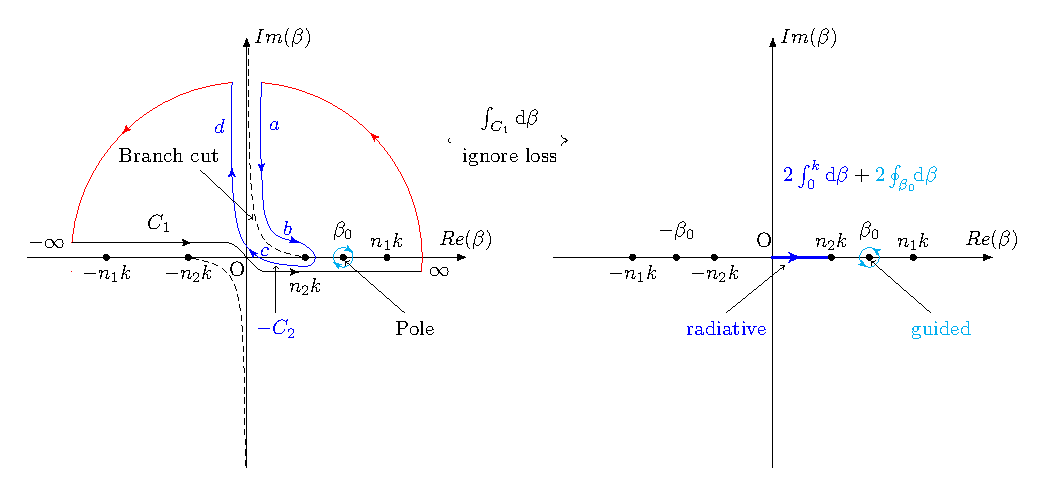
\includegraphics[scale=0.75]{./Figs/contourplot_upper}}
\end{minipage}
\par\medskip
\begin{minipage}{.91\linewidth}
\centering
\subfloat[]{\label{contourplot_lower}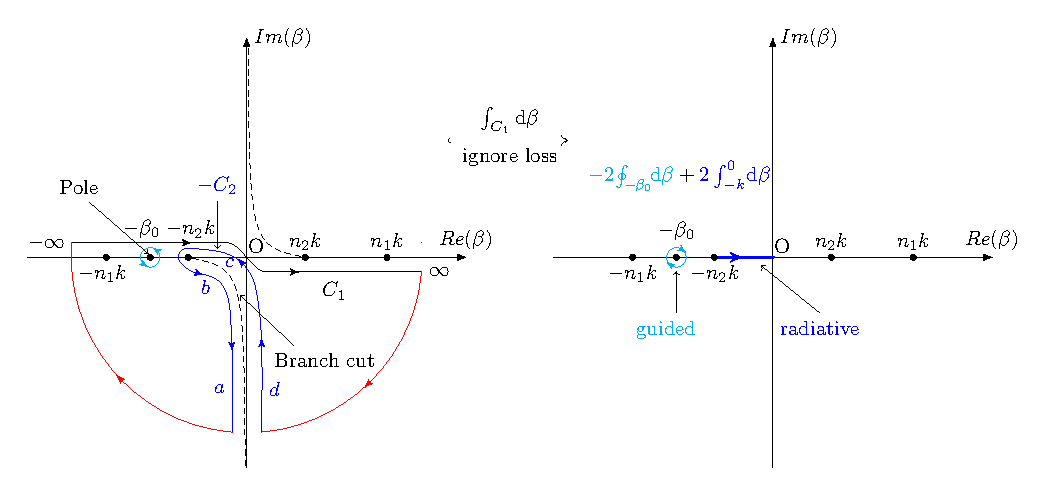
\includegraphics[scale=0.75]{./Figs/contourplot_lower}}
\end{minipage}
\caption{Equivalent integration paths to calculate the radiation and guided fields. For $ z>0 $, we can use the zero-valued contour integral path drawn in subfig.~\ref{contourplot_upper} to calculate the integration along path $ C_1 $. The simplified integration path by ignoring waveguide losses is given on the right-hand-side. It only contains the forward propagating mode contributions with radiation and guided mode components as divided through the real-axis integral and the loop-hole integral. For the $ z<0 $ case, the contour integral analysis is given in subfig.~\ref{contourplot_lower}, which only includes the backward propagating mode contributions.}
\label{fig:integralpath}
\end{figure}

\textcolor{blue}{More information: Physics meaning of the sections detouring the branch cuts and poles...} The integrals along the vertical sections of the contour paths, $ a $ and $ d $, cancel. The integrals along the horizontal sections, $ b $ and $ c $, double one the other. In the end, the contour integral detouring the branch cuts yields $ 2\int_0^k\mathrm{d}\beta $ for $ z>0 $ or $ 2\int_{-k}^0\mathrm{d}\beta $ for $ z<0 $ with $ n_2=1 $. Similarly, one can show that the contour integrals around the poles with separated segments of positive and negative real $ p $'s are equivalent to $ \pm 2\oint_{\pm \beta_0}\!\!\mathrm{d}\beta $ with positive real $ p $. When $ z=0 $, the full integral along path $ C_1 $ can be rewritten as the average value of the $ z>0 $ and $ z<0 $ limits. Therefore, we have 
\begin{align}
\int_{C_1}\mathrm{d}\beta =\int_{-k}^k\mathrm{d}\beta +\oint_{\beta_0}\mathrm{d}\beta -\oint_{-\beta_0}\!\!\mathrm{d}\beta,
\end{align}
where the first integral yield the radiation mode contribution and the last two terms yield the guided mode contribution in two respective propagation directions. When we calculate the decay rates or phase shift due to the presence of atoms, we can use this decomposition relationship of integrals. Notice that, the guided mode contribution part should only include the $ m=\pm 1 $ $\mathrm{HE}_{11}$ modes when summing over mode index $ m $ for a single-mode nanofiber. 



\section{Group index of refraction and mode functions of the fundamental guided modes}
The longitudinal propagation constant $\beta$ of the fundamental $\mathrm{HE}_{11}$ guided mode is determined by the fiber eigenvalue equation~\cite{LeKien2005}
\begin{align}
f(h,q,k,\beta) &=0,
\end{align}
where
\begin{align}
f(h,q,k,\beta) &=\frac{J_0(ha)}{haJ_1(ha)}+\frac{n_1^2+n_2^2}{2n_1^2}\frac{K_1^\prime(qa)}{qaK_1(qa)}-\frac{1}{h^2a^2} \\
&+\left\{\left[\frac{n_1^2-n_2^2}{2n_1^2}\frac{K_1^\prime(qa)}{qaK_1(qa)} \right]^2 +\frac{\beta^2}{n_1^2k^2}\left(\frac{1}{q^2a^2}+\frac{1}{h^2a^2} \right)^2 \right\}^{1/2}
\end{align}
and the transverse propagation parameters $h=\sqrt{n_1^2k^2-\beta^2}$ and $q=\sqrt{\beta^2-n_2^2k^2}=\sqrt{\beta^2-k^2}$. $J_n$ and $K_n$ stand for the Bessel functions of the first kind and the modified Bessel functions of the second kind, respectively. 

We differentiate the fiber eigenvalue equation above with respect to $ \beta $ on both sides, and obtain
\begin{align}
\dd{f}{\beta} &= \pp{f}{h} \left(\pp{h}{k}\dd{k}{\beta}+\pp{h}{\beta} \right) + \pp{f}{q}\left(\pp{q}{k}\dd{k}{\beta}+\pp{q}{\beta} \right) +\pp{f}{k}\dd{k}{\beta}+\pp{f}{\beta}=0
\end{align}
Therefore, the group index of refraction of the fundamental modes of the nanofiber can be given by
\begin{align}
 n_g &= \dd{\beta}{k} = -\frac{\pp{f}{h}\pp{h}{k}+\pp{f}{q}\pp{q}{k}+\pp{f}{k}}
{\pp{f}{h}\pp{h}{\beta}+\pp{f}{q}\pp{q}{\beta}+\pp{f}{\beta}}.
\end{align}

\todo[inline]{Frequency stability, linearity and such of the group index of refraction.}

The fundamental mode functions, $\mathbf{u}^{(\mu)}(r\!_\perp,\phi,z)$, of the electric components of the fiber~\cite{LeKien2005,Lacroute2012} can be separated into $r\!_\perp-$, $\phi-$ and $z-$ dependent parts, and are characterized by the mode index $\mu=(\omega,f,\xi)$, where $f=\pm 1$ indicates forward and backward propagating directions and $\xi $ indicates the polarization state of the mode. For a quasicircularly polarized fundamental mode, we use $\xi=m=\pm $ to indicate the counterclockwise and clockwise rotations, respectively; for a quasilinearly polarized fundamental mode, we usually use $\xi=\phi_0$ to indicate the polarization axis is rotated by $\phi_0$ from the $x$-axis; specially, we use $\xi=H$ or $V$ when the quasilinear polarization axis is along the $x$-axis or $y$-axis, respectively. For the circularly polarized case, the fundamental mode can be written as 
\begin{align}
\mathbf{u}^{(\mu)}(r\!_\perp,\phi,z) &=u^{(\mu)}_{r\!_\perp}(r\!_\perp) e^{if\beta z+im\phi }\hat{r}\!_\perp +u^{(\mu)}_{\phi}(r\!_\perp) e^{if\beta z+im\phi } \hat{\phi} +u^{(\mu)}_{z}(r\!_\perp)e^{if\beta z+im\phi }\hat{z}\\
&=u_{r\!_\perp}(r\!_\perp) e^{if\beta z+im\phi }\hat{r}\!_\perp + m u_{\phi}(r\!_\perp) e^{if\beta z+im\phi }\hat{\phi} + f u_z (r\!_\perp) e^{if\beta z+im\phi }\hat{z},
\end{align}
where the forwarding, counterclockwise rotating guided mode components, $\mathbf{u}(r\!_\perp)$, are determined, for $r\!_\perp<a$, by
\begin{subequations}
\label{urtcrla}
\begin{align}
u_{r\!_\perp}(r\!_\perp) &=iA\frac{\beta_0}{2h} \left[ (1-s)J_0(hr\!_\perp)-(1+s)J_2(hr\!_\perp) \right]\\
u_\phi(r\!_\perp) &=  -mA \frac{\beta_0}{2h} \left[ (1-s)J_0(hr\!_\perp) +(1+s)J_2(hr\!_\perp) \right] \\
u_z(r\!_\perp) &= fA J_1(hr\!_\perp),
\end{align}
\end{subequations}
and, for $ r_\perp>a $, by
\begin{subequations}
\label{urtcrga}
\begin{align}
u_{r\!_\perp}(r\!_\perp) &=iA\frac{\beta_0}{2h}\frac{J_1(ha)}{K_1(qa)} \left[ (1-s)K_0(qr\!_\perp)+(1+s)K_2(qr\!_\perp) \right]\\
u_\phi(r\!_\perp) &=  -mA \frac{\beta_0}{2h} \frac{J_1(ha)}{K_1(qa)} \left[ (1-s)K_0(qr\!_\perp) - (1+s)K_2(qr\!_\perp) \right] \\
u_z(r\!_\perp) &= fA \frac{J_1(ha)}{K_1(qa)} K_1(qr\!_\perp),
\end{align}
\end{subequations}
with
\begin{align}
s &= \left[\frac{1}{(ha)^2}+ \frac{1}{(qa)^2} \right] \left[ \frac{J_1'(ha)}{haJ_1(ha)} + \frac{K'_1(qa)}{qaK_1(qa)} \right],\\
h &= \sqrt{k^2 n_1^2-\beta_0^2}.
\end{align}
The normalization factor, $A$, is determined by the normalized energy that 
\begin{align}
1 &= \int_0^{2\pi} \!\!\mathrm{d} \phi \int_0^\infty\!\!\mathrm{d}r\!_\perp r\!_\perp\,  n^2(\br\!_\perp)|\boldsymbol{\mathcal{E}}^g(\br\!_\perp)|^2 = 2\pi A^2 a^2 (n_1^2P_1 + n_2^2P_2),
\end{align}
where the stored energy distribution factors are given by
\begin{align}
\!\!\!\!\! P_1
&= \frac{\beta^2}{4h^2}\!\left\{(1\!-\! s)^2\!\left[J_0^2(ha)\!+\! J_1^2(ha) \right] \!+\!(1\!+\!s)^2\!\left[J_2^2(ha)\!-\!J_1(ha)J_3(ha) \right]\right\}\nonumber\\
&\quad +\frac{1}{2}\left[J_1^2(ha)-J_0(ha)J_2(ha) \right] \\
\!\!\!\!\! P_2
&= \frac{\beta^2J_1^2(ha)}{4q^2K_1^2(qa)}\!\left\{\phantom{\frac{1}{1}}\!\!\!\!(1\!-\!s)^2\!\left[K_1^2(qa)\!-\!K_0^2(qa) \right]\right.\nonumber\\
&\quad\left. \!+(1\!+\!s)^2\!\!\left[K\!_1\!(qa)K\!_3\!(qa)\!-\! K_2^2\!(qa) \right]\!+\!\frac{2q^2}{\beta^2}\!\!\left[K\!_0\!(qa)K\!_2\!(qa)\!-\!K_1^2\!(qa) \right]  \right\}.
\end{align}
Using this basis, the electric part of a guided field with quasicircularly propagating mode index $\mu=(\omega f m)$ can be written as 
\begin{align}
E^{(\mu)}(r\!_\perp,\phi,z,t) &=E_0(u_{r\!_\perp}(r\!_\perp) e^{if\beta z+im\phi-i\omega t }\hat{r}\!_\perp + m u_{\phi}(r\!_\perp) e^{if\beta z+im\phi-i\omega t }\hat{\phi} + f u_z (r\!_\perp) e^{if\beta z+im\phi-i\omega t }\hat{z}).
\end{align}
By using the power propagating inside and outside the fiber can be given in terms of the time averaged Poynting vector along the propagation direction, $\left< S_z \right>$, by
\begin{align}
P_{in} &= \int_0^{2\pi} \mathrm{d}\phi \int_0^a \left< S_z \right> r\!_\perp \mathrm{d}r\!_\perp\\
P_{out} &= \int_0^{2\pi} \mathrm{d}\phi \int_a^\infty \left< S_z \right> r\!_\perp \mathrm{d}r\!_\perp,
\end{align}
and the total power $ P=P_{in}+P_{out} $, one can show that the normalization constant $ E_0 A $ reads
\begin{align}\label{eq:EA}
E_0 A=\sqrt{\frac{4\mu_0\omega P}{\pi a^2 \beta_0}}\left(D_{in} + D_{out} \right)^{-1/2},
\end{align}
where
\begin{align}
D_{in} &= (1-s)\left[ 1+(1-s)\frac{\beta_0^2}{h^2}\right] \left(J_0^2(ha) + J_1^2(ha) \right) \nonumber\\
&\quad + (1+s)\left[ 1+(1+s)\frac{\beta_0^2}{h^2}\right] \left(J_2^2(ha)- J_1(ha)J_3(ha) \right)\\
D_{out} &= \frac{J_1^2(ha)}{K_1^2(qa)}\left\{ (1-s)\left[ 1-(1-s)\frac{\beta_0^2}{q^2}\right] \left(K_0^2(qa) - K_1^2(qa) \right)\right. \nonumber\\
&\quad \left. + (1\!+\! s)\left[ 1\!-\! (1\!+\! s)\frac{\beta_0^2}{q^2}\right] \left(K_2^2(qa)\! -\! K_1(qa)K_3(qa) \right) \right\}.
\end{align}



For a quasilinearly polarized fundamental guided mode, the electric part of the mode can be written as 
\begin{align}
\mathbf{u}^{(\omega f \phi_0)}(r\!_\perp,\phi,z) &= \frac{1}{\sqrt{2}} \left(\mathbf{u}^{(\omega f +)}(r\!_\perp,\phi,z)e^{-i\phi_0} +\mathbf{u}^{(\omega f -)}(r\!_\perp,\phi,z)e^{i\phi_0} \right)\\
&= \sqrt{2}\left[u_{r\!_\perp}(r\!_\perp)\cos(\phi-\phi_0)\hat{\mathbf{r}}\!_\perp + iu_\phi(r\!_\perp)\sin(\phi-\phi_0)\hat{\boldsymbol{\phi}} \right. \nonumber \\
&\quad\quad \left. + fu_z(r\!_\perp)\cos(\phi-\phi_0)\hat{\mathbf{z}} \right]e^{if\beta z}.
\end{align}
One can write down an arbitrary quasilinearly polarized electric field in the form similar to the quasicircularly polarized case with $E_0A$ satisfying the same relationship defined in Equ.~\eqref{eq:EA}. 

Particularly, when $\phi_0=0$ and $\pi/2$, we obtain the $H$ and $V$ fundamental modes as given by
\begin{align}
\mathbf{u}^{(\omega f H)}(r\!_\perp,\phi,z)
&= \sqrt{2}\left[u_{r\!_\perp}(r\!_\perp)\cos(\phi)\hat{\mathbf{r}}\!_\perp + iu_\phi(r\!_\perp)\sin(\phi)\hat{\boldsymbol{\phi}} + fu_z(r\!_\perp)\cos(\phi)\hat{\mathbf{z}} \right]e^{if\beta z}\\
\mathbf{u}^{(\omega f V)}(r\!_\perp,\phi,z)
&= \sqrt{2}\left[u_{r\!_\perp}(r\!_\perp)\sin(\phi)\hat{\mathbf{r}}\!_\perp - iu_\phi(r\!_\perp)\cos(\phi)\hat{\boldsymbol{\phi}}  + fu_z(r\!_\perp)\sin(\phi)\hat{\mathbf{z}} \right]e^{if\beta z}.
\end{align}

\todo[inline]{To show $v_g=\frac{P}{W}$ using the formulas above?}



\section{Junk: Effects of the evanescent field and the multilevel structure of the atom}
In general, 
\begin{align}
\Gamma \propto \mathbf{d}_{eg}\cdot \mathrm{Im}\left[\mathbf{G}(\br',\br') \right]\cdot\mathbf{d}_{eg}^*=\mathrm{tr}\left[\mathbf{d}_{eg}^*\mathbf{d}_{eg}\cdot \mathrm{Im}\left[\mathbf{G}(\br',\br') \right] \right]\propto \mathrm{tr}\left[\boldsymbol{\alpha}_{eg}\cdot \mathrm{Im}\left[\mathbf{G}(\br',\br') \right] \right]
\end{align}
where $ \boldsymbol{\alpha}_{eg} $ is the polarizability of the atom due to the transition between levels labeled by $ eg $. Therefore, the phase shift effect can be treated as a combination effect of the atomic internal structure and the external field properties. 

Since 
\begin{align}
\mathbf{d}_{eg}\cdot \mathrm{Im}\left[\mathbf{G}(\br',\br') \right]\cdot\mathbf{d}_{eg}^*>0
\end{align}
for a physical decay rate, $\mathrm{Im}\left[\mathbf{G}(\br',\br')\right]$ is positive definite and should always has three positive eigenvalues which indicate the range of $ \Gamma $ and phase shift at the atom position. The 3 corresponding eigenvectors indicate the 3 orthogonal principal axes of the radiation/emission surface. Case studies...

Radiation surface theory for the effective orientation of dipoles, elementary transitions ($ \pi $ and $ \sigma_\pm $ transitions) and the example of completely mixed state case. 
\begin{align}
\Gamma_{mix} &\propto \frac{1}{3} \mathrm{tr}\left[ \mathrm{Im}\left[\mathbf{G}(\br',\br')\right] \right].
\end{align}

For the atomic internal structure, we have the irreducible tensor decompositions that 
\begin{align}
\boldsymbol{\alpha}_{eg} = \boldsymbol{\alpha}^S + \boldsymbol{\alpha}^V + \boldsymbol{\alpha}^T.
\end{align}
The scalar component will yield a decay rate equivalent to the completely mixed state case. 

Another way to look at this problem is that we can decompose the guided mode Green function tensor into the scalar, vector and tensor parts as well, since it is irreducible.
\begin{align}
\mathbf{G}^g=\mathbf{G}^S+\mathbf{G}^V+\mathbf{G}^T.
\end{align}
Therefore, where the position of the atom relative to the fiber mode yields a strong scalar component, the atomic response is more independent of the atom state... 

Some interesting examples of state-dependent decay and phase shift...


%\begin{center}
%{\bf References}
%\end{center}

%\bibliography
%\bibliographystyle{amsplain}
\bibliographystyle{unsrt}
% \nocite{*}
\ifwindows
	\bibliography{F:/References/Archive/Archive}
\else
	\bibliography{/media/F/References/Archive/Archive}
\fi


\end{document}